
%\setcounter{chapter}{6}

\chapter{Introduction to Learning}
\label{chapter:intro_to_learning}

\section{Introduction}
The goal of learning is to extract lessons from past experience in order to solve future problems. Typically, this involves searching for an algorithm that solves past instances of the problem. This algorithm can then be applied to future instances of the problem.

\marginnote{Past and future do not necessarily refer to the calendar date; instead they refer to what the \textit{learner} has previously seen and what the learner will see next.}[-1.4cm]
%\marginnote{An {\bf algorithm} is a formal mapping from inputs to outputs, e.g., from a problem statement to its solution.}[-0.83cm]

Because learning is itself an algorithm, it can be understood as a meta-algorithm: an algorithm that outputs algorithms (\fig{\ref{fig:learning_as_meta_algorithm}}).

\begin{figure}[h!]
    \centerline{
    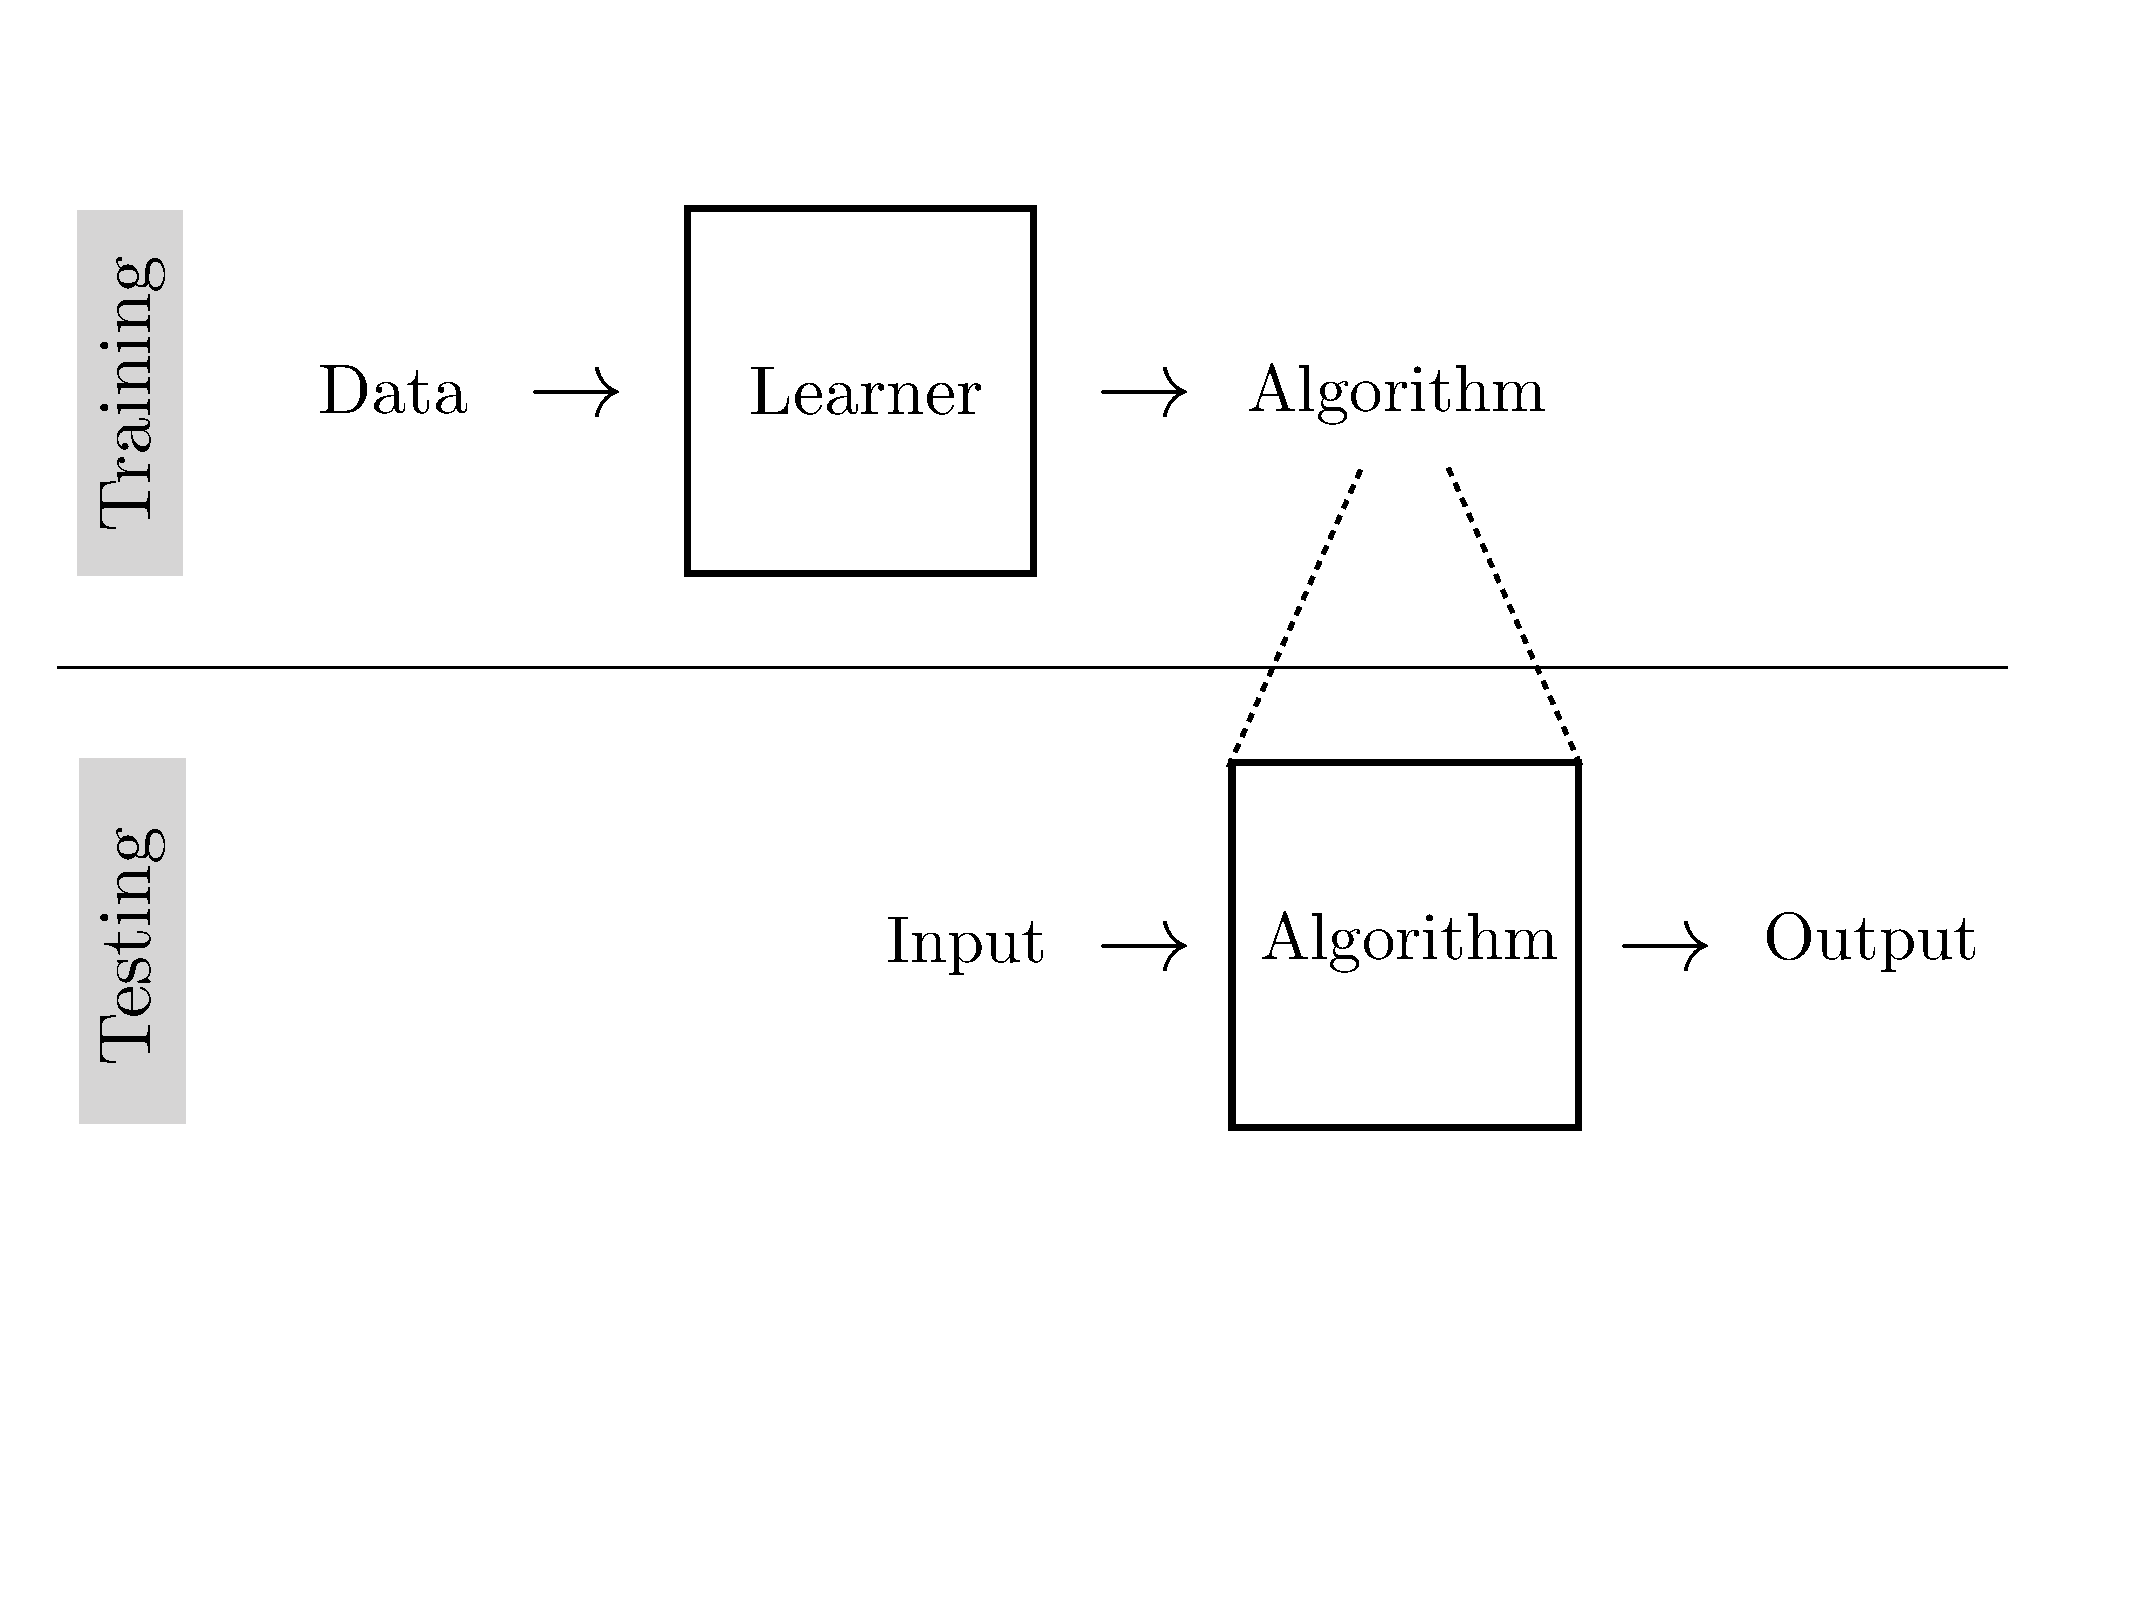
\includegraphics[width=0.75\linewidth]{./figures/intro_to_learning/learning_as_meta_algorithm.pdf}
    }
    \caption{Learning is an algorithm that outputs algorithms.}
    \label{fig:learning_as_meta_algorithm}
\end{figure}

Learning usually consists of two phases: the \index{Training phase}{\bf training} phase, where we search for an algorithm that performs well on past instances of the problem (training data), and the \index{Testing phase}{\bf testing} phase, where we deploy our learned algorithm to solve new instances of the problem.

%What exactly is an instance of a ``problem"? A common definition is a \{\texttt{question}, \texttt{answer}\} pair. Solving the problem consists of providing the \texttt{answer} to the \texttt{question}. From this perspective, a machine learning algorithm produces a set of rules that map \texttt{questions} to \texttt{answers}. A more general way to think of it is a machine learning algorithm produces a mapping from \texttt{inputs} to desirable \texttt{outputs}.

\section{Learning from Examples}
\marginnote{Learning from examples is also called \textbf{supervised learning}.}[-0.6cm]

%\marginnote{Learning from examples is sometimes called {\bf supervised learning}.}[-0.83cm]

Imagine you find an ancient mathematics text, with marvelous looking proofs, but there is a symbol you do not recognize, ``$\star$". You see it being used here and there in equations, and you note down examples of its behavior:
\begin{align}
    2 \star 3 &= 36\nonumber \\
    7 \star 1 &= 49\nonumber \\
    5 \star 2 &= 100\nonumber \\
    2 \star 2 &= 16\nonumber
\end{align}
What do you think $\star$ represents? What function is it computing? Do you have it? Let's test your answer: what is the value of $3 \star 5$? (The answer is in the figure below.)

It may not seem like it, but you just performed learning! You \emph{learned} what $\star$ does by looking at examples. In fact, \fig{\ref{fig:star_symbol_learning}} shows what you did:

\begin{figure}[h]
    \centerline{
    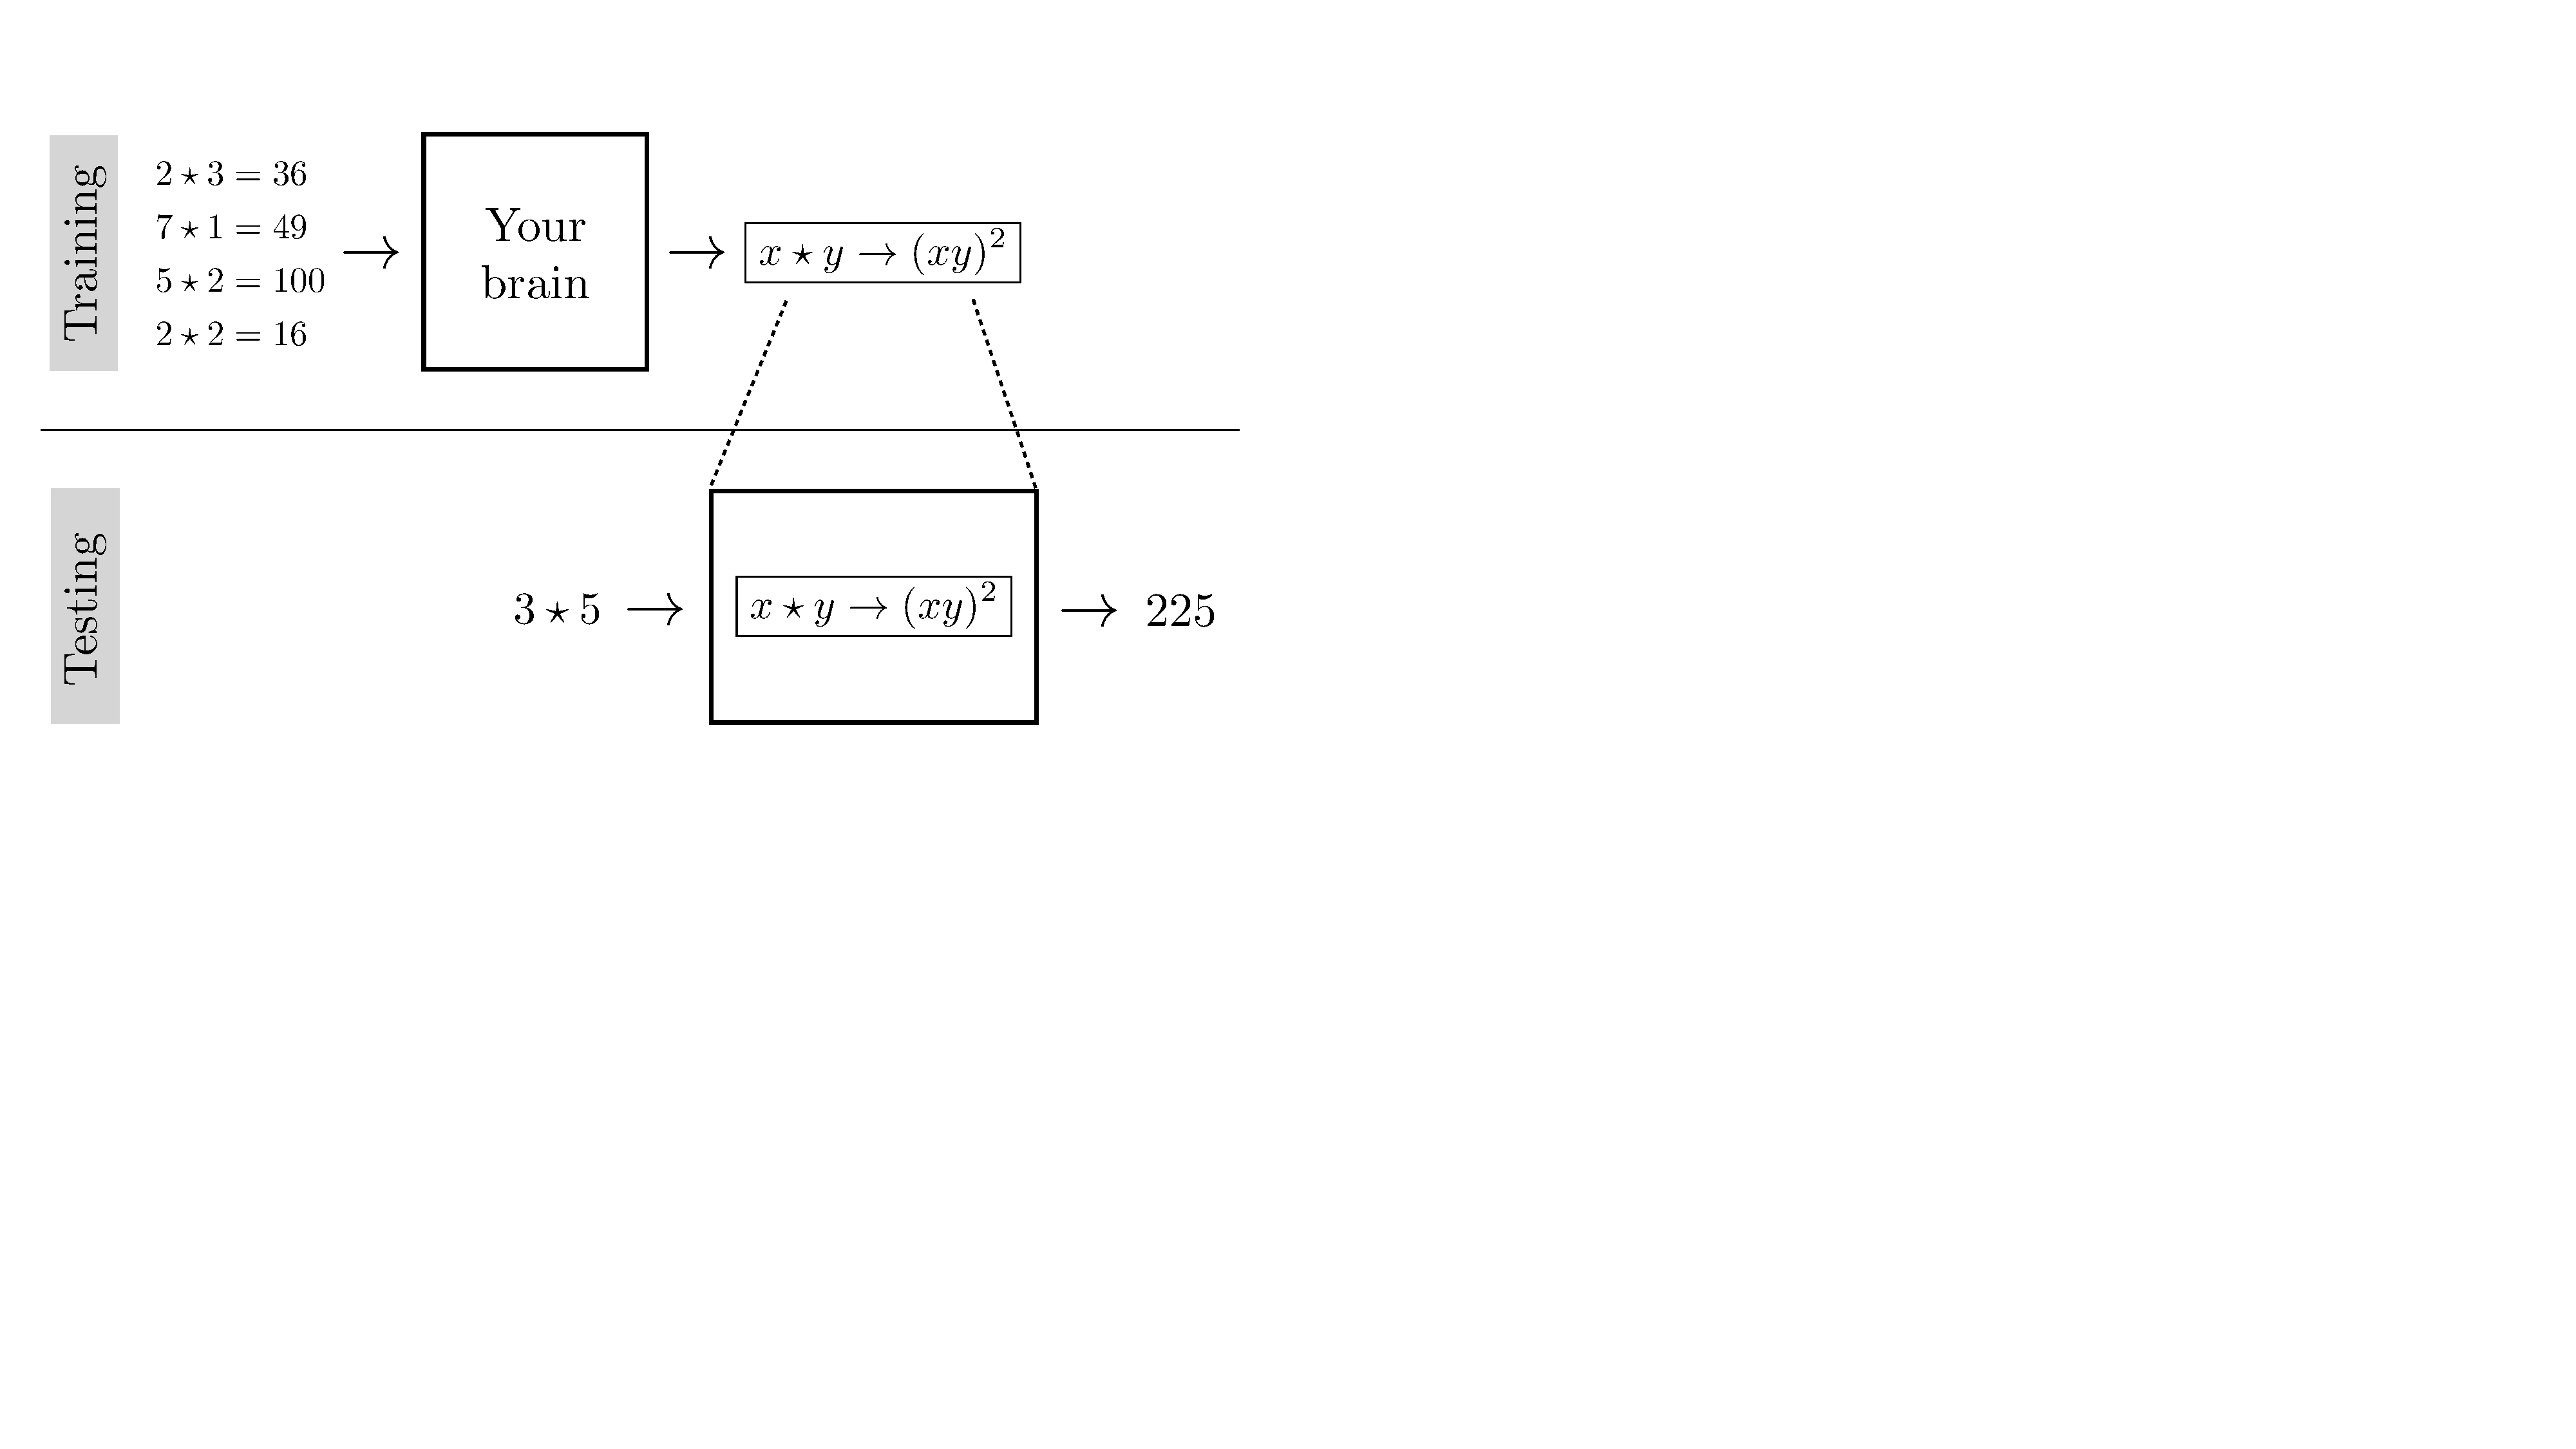
\includegraphics[width=0.75\linewidth]{./figures/intro_to_learning/star_symbol_learning.pdf}
    }
    \caption{How your brain may have solved the star problem.}
    \label{fig:star_symbol_learning}
\end{figure}

Nice job!

It turns out, we can learn almost anything from examples. 
Remember that we are learning an \emph{algorithm}, i.e., a computable mapping from inputs to outputs. A formal definition of \emph{example}, in this context, is an \{\texttt{input}, \texttt{output}\} pair. The examples you were given for $\star$ consisted of four such pairs:
\begin{align}
    &\{\texttt{input:} [2,3], \texttt{output:} 36\}\nonumber \\
    &\{\texttt{input:} [7,1], \texttt{output:} 49\}\nonumber \\
    &\{\texttt{input:} [5,2], \texttt{output:} 100\}\nonumber \\
    &\{\texttt{input:} [2,2], \texttt{output:}16\}\nonumber
\end{align}
This kind of learning, where you observe example input-output behavior and infer a functional mapping that explains this behavior, is called \index{Supervised learning}\textbf{supervised learning}. 

\marginnote{Another name for this kind of learning is {\bf fitting a model} to data.}[-1cm]

We were able to model the behavior of $\star$, on the examples we were given, with a simple algebraic equation. Let's try something rather more complicated. From the three examples in \fig{\ref{fig:intro_to_learning:inpainting_example}}, can you figure out what the operator $F$ does?

\begin{figure}[h]
    \centerline{
    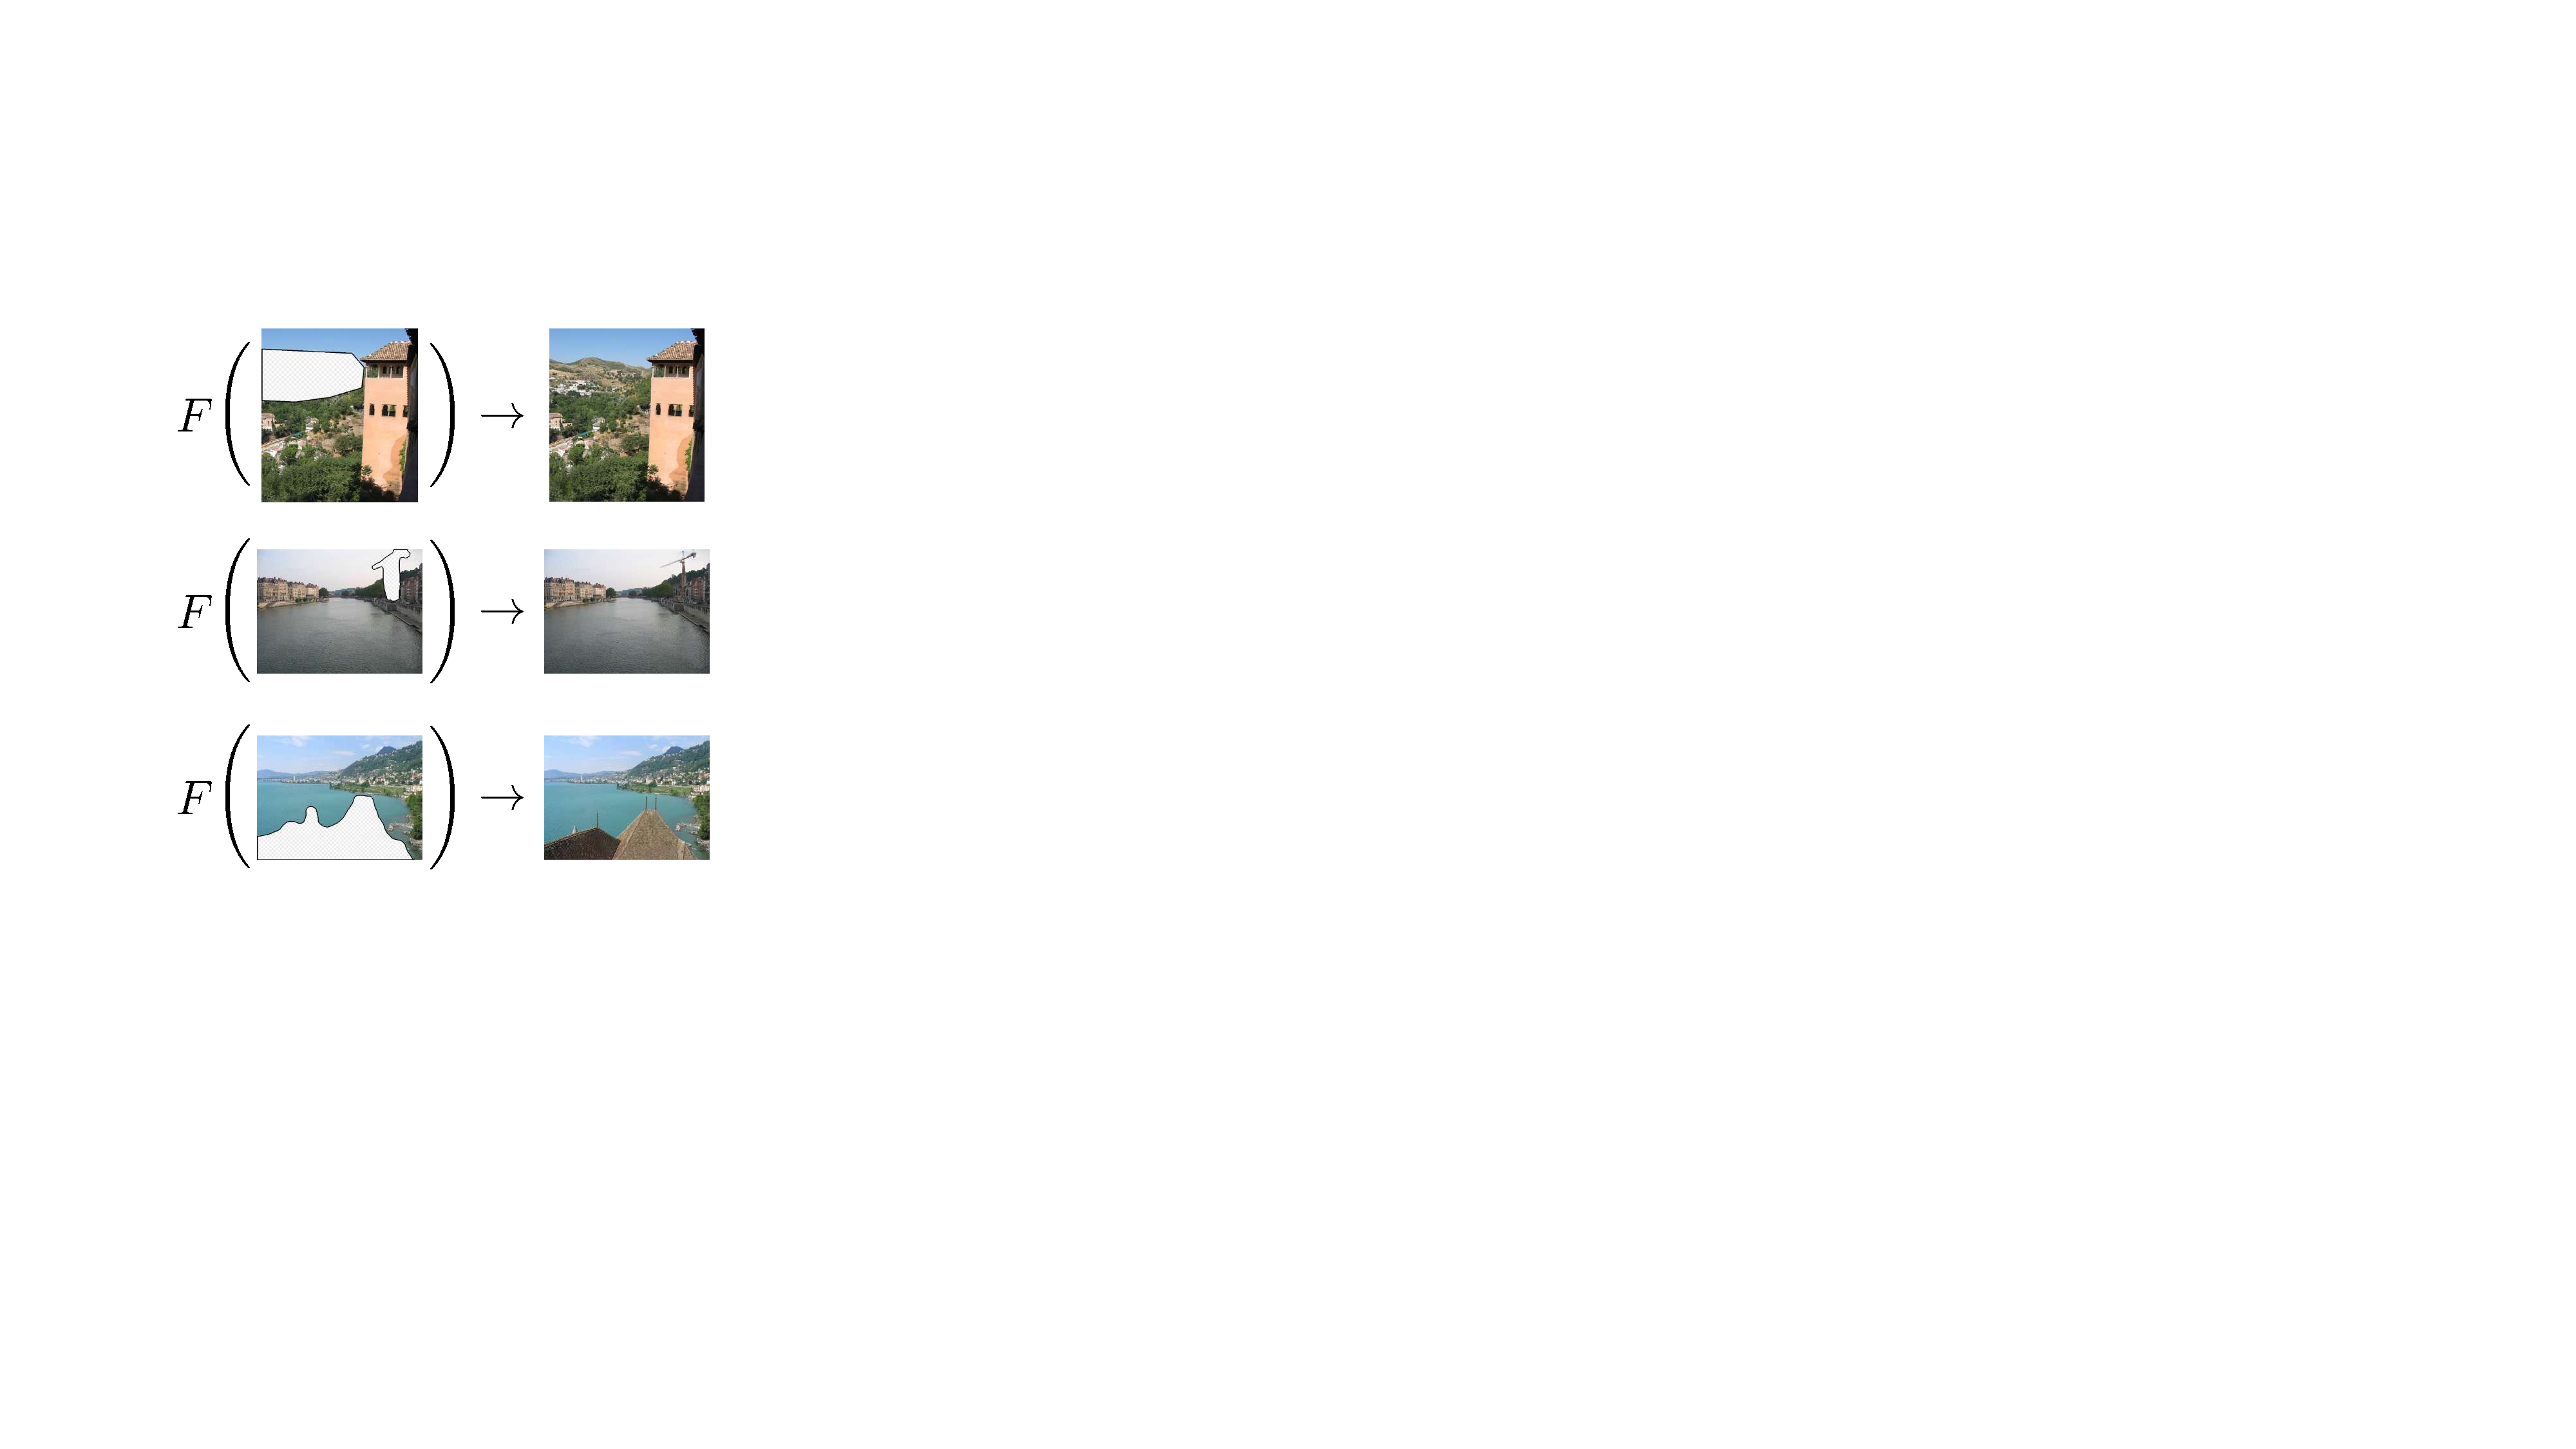
\includegraphics[width=0.4\linewidth]{./figures/intro_to_learning/inpainting_example.pdf}
    }
    \caption{A complicated function that could be learned from examples. This example is from \cite{hays2007scene}. \reviewcomment{Get permission}}
    \label{fig:intro_to_learning:inpainting_example}
\end{figure}

You probably came up with something like ``it fills in the missing pixels.'' That's exactly right, but it's sweeping a lot of details under the rug. Remember, we want to learn an \emph{algorithm}, a procedure that is completely unambiguous. How exactly does $F$ fill in the missing pixels? 

It's hard to say in words. We may need a very complex algorithm to specify the answer, an algorithm so complex that we could never hope to write it out by hand. This is the point of machine learning. The machine writes the algorithm for us, but it can only do so if we give it many examples, not just these three.

\marginnote{Some things are not learnable from examples, such as noncomputable functions. An example of a noncomputable function is a function that takes as input a program and outputs a 1 if the program will eventually finish running, and a 0 if it will run forever. It is noncomputable because there is no algorithm that can solve this task in finite time. However, it might be possible to learn a good approximation to it.}[-.7in] 

\section{Learning without Examples}
%\marginnote{Methods for learning without examples include \textbf{unsupervised learning} and \textbf{reinforcement learning}.}

Even without examples, we can still learn. Instead of matching input-output examples, we can try to come up with an algorithm that optimizes for desirable \emph{properties} of the input-output mapping. This class of learners includes \index{Unsupervised learning}{\bf unsupervised learning} and \index{Reinforcement learning}{\bf reinforcement learning}. 

%In both of these frameworks, we are given an \textbf{objective function} that scores the quality of the learned function's output.

In unsupervised learning, we are given examples of \textit{input data} $\{x^{(i)}\}^N_{i=1}$ but we are not told the target outputs $\{y^{(i)}\}^N_{i=1}$. Instead the learner has to come up with a model or representation of the input data that has useful properties, as measured by some \textbf{objective function}. The objective could be, for example, to compress the data into a lower dimensional format that still preserves all information about the inputs. We will encounter this kind of learning in \partref{\ref{part:generative_models_and_representation_learning}} of this book, on representation learning and generative modeling.

In reinforcement learning, we suppose that we are given a 
\index{Reward function}{\bf reward function} that explicitly measures the quality of the learned function's output. To be precise, a reward function is a mapping from outputs to scores: $r: \mathcal{Y} \rightarrow \mathbb{R}$. The learner tries to come up with a function that maximizes rewards. This book will not cover reinforcement learning in detail, but this kind of learning is becoming an important part of computer vision, especially in the context of vision for robots. We direct the interested reader to \cite{sutton2018reinforcement} to learn more.%Reinforcement learning also usually deals with the setting where the learned function gets to pick which training datapoints to observe next, rather than being provided them passively. An example is an agent that chooses which actions to take as it navigates a room, and this choice of action determines what data (view of the world) the agent will next observe. This dependence of data on learned function is one of the main reasons reinforcement learning is hard.
\marginnote{At first glance unsupervised learning and reinforcement learning look similar: both maximize a function that scores desirable properties of the input-output mapping. The big difference is that unsupervised learning has access to \textit{training data} whereas reinforcement learning usually does not; instead the reinforcement learner has to collect its own training data.}[-5cm]


\section{Key Ingredients}
\label{sec:intro_to_learning:key_ingredients}

A learning algorithm consists of three key ingredients:
\begin{enumerate}
    \item \index{Objective function}{\bf Objective}: What does it mean for the learner to succeed, or, at least, to perform well? 
    \item \index{Hypothesis space}{\bf Hypothesis space}: What is the set of possible mappings from inputs to outputs that we will we search over?
    \item \index{Optimizer}{\bf Optimizer}: \emph{How}, exactly, do we search the hypothesis space for a specific mapping that maximizes the objective?
\end{enumerate}
%\marginnote{These three ingredients will help organize our thinking in this book, but they are not meant to be comprehensive. In particular, we can drill down into any one of these categories and find interesting additional choices. For example, after choosing a hypothesis space, the next critical decision is how to \textit{parameterize} the hypothesis space. We discuss this choice in Section XX.}

These three ingredients, when applied to large amounts of data, and run on sufficient hardware (referred to as {\bf compute}) can do amazing things. We will focus on the learning algorithms in this chapter, but often the data and compute turn out to be more important.

\begin{center}
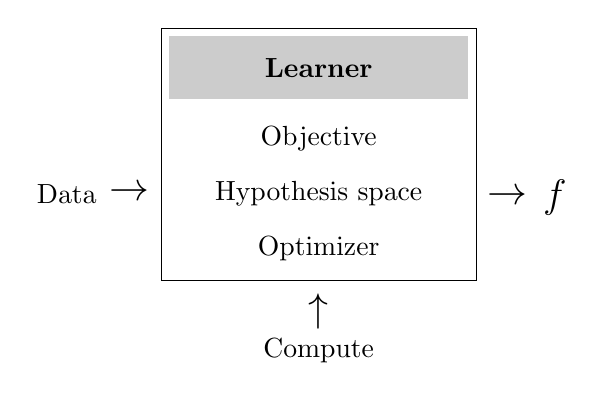
\begin{tikzpicture}
    \draw (0,0) rectangle (4,3.2); % outer box
    \fill[black!20] (0.1,2.3) rectangle (3.9,3.1); % gray box
    \node[] at (2,2.7) {{\bf Learner}};
    \node[] at (2,1.8) {Objective};
    \node[] at (2,1.1) {Hypothesis space};
    \node[] at (2,0.4) {Optimizer};
    \node[] at (-1.2,1.1) {Data};
    \node[] at (-0.4,1.1) {{\Large  $ \rightarrow$}};
    \node[] at (5,1.05) {{\Large $f$}};
    \node[] at (4.4,1.05) {{\Large  $ \rightarrow$}};
    \node[] at (2,-0.4) {{\Large  $ \uparrow$}};
    \node[] at (2,-0.9) {Compute};
\label{fig:ingredients}
\end{tikzpicture}
\end{center}

% \begin{figure}[h]
%     \centering
%     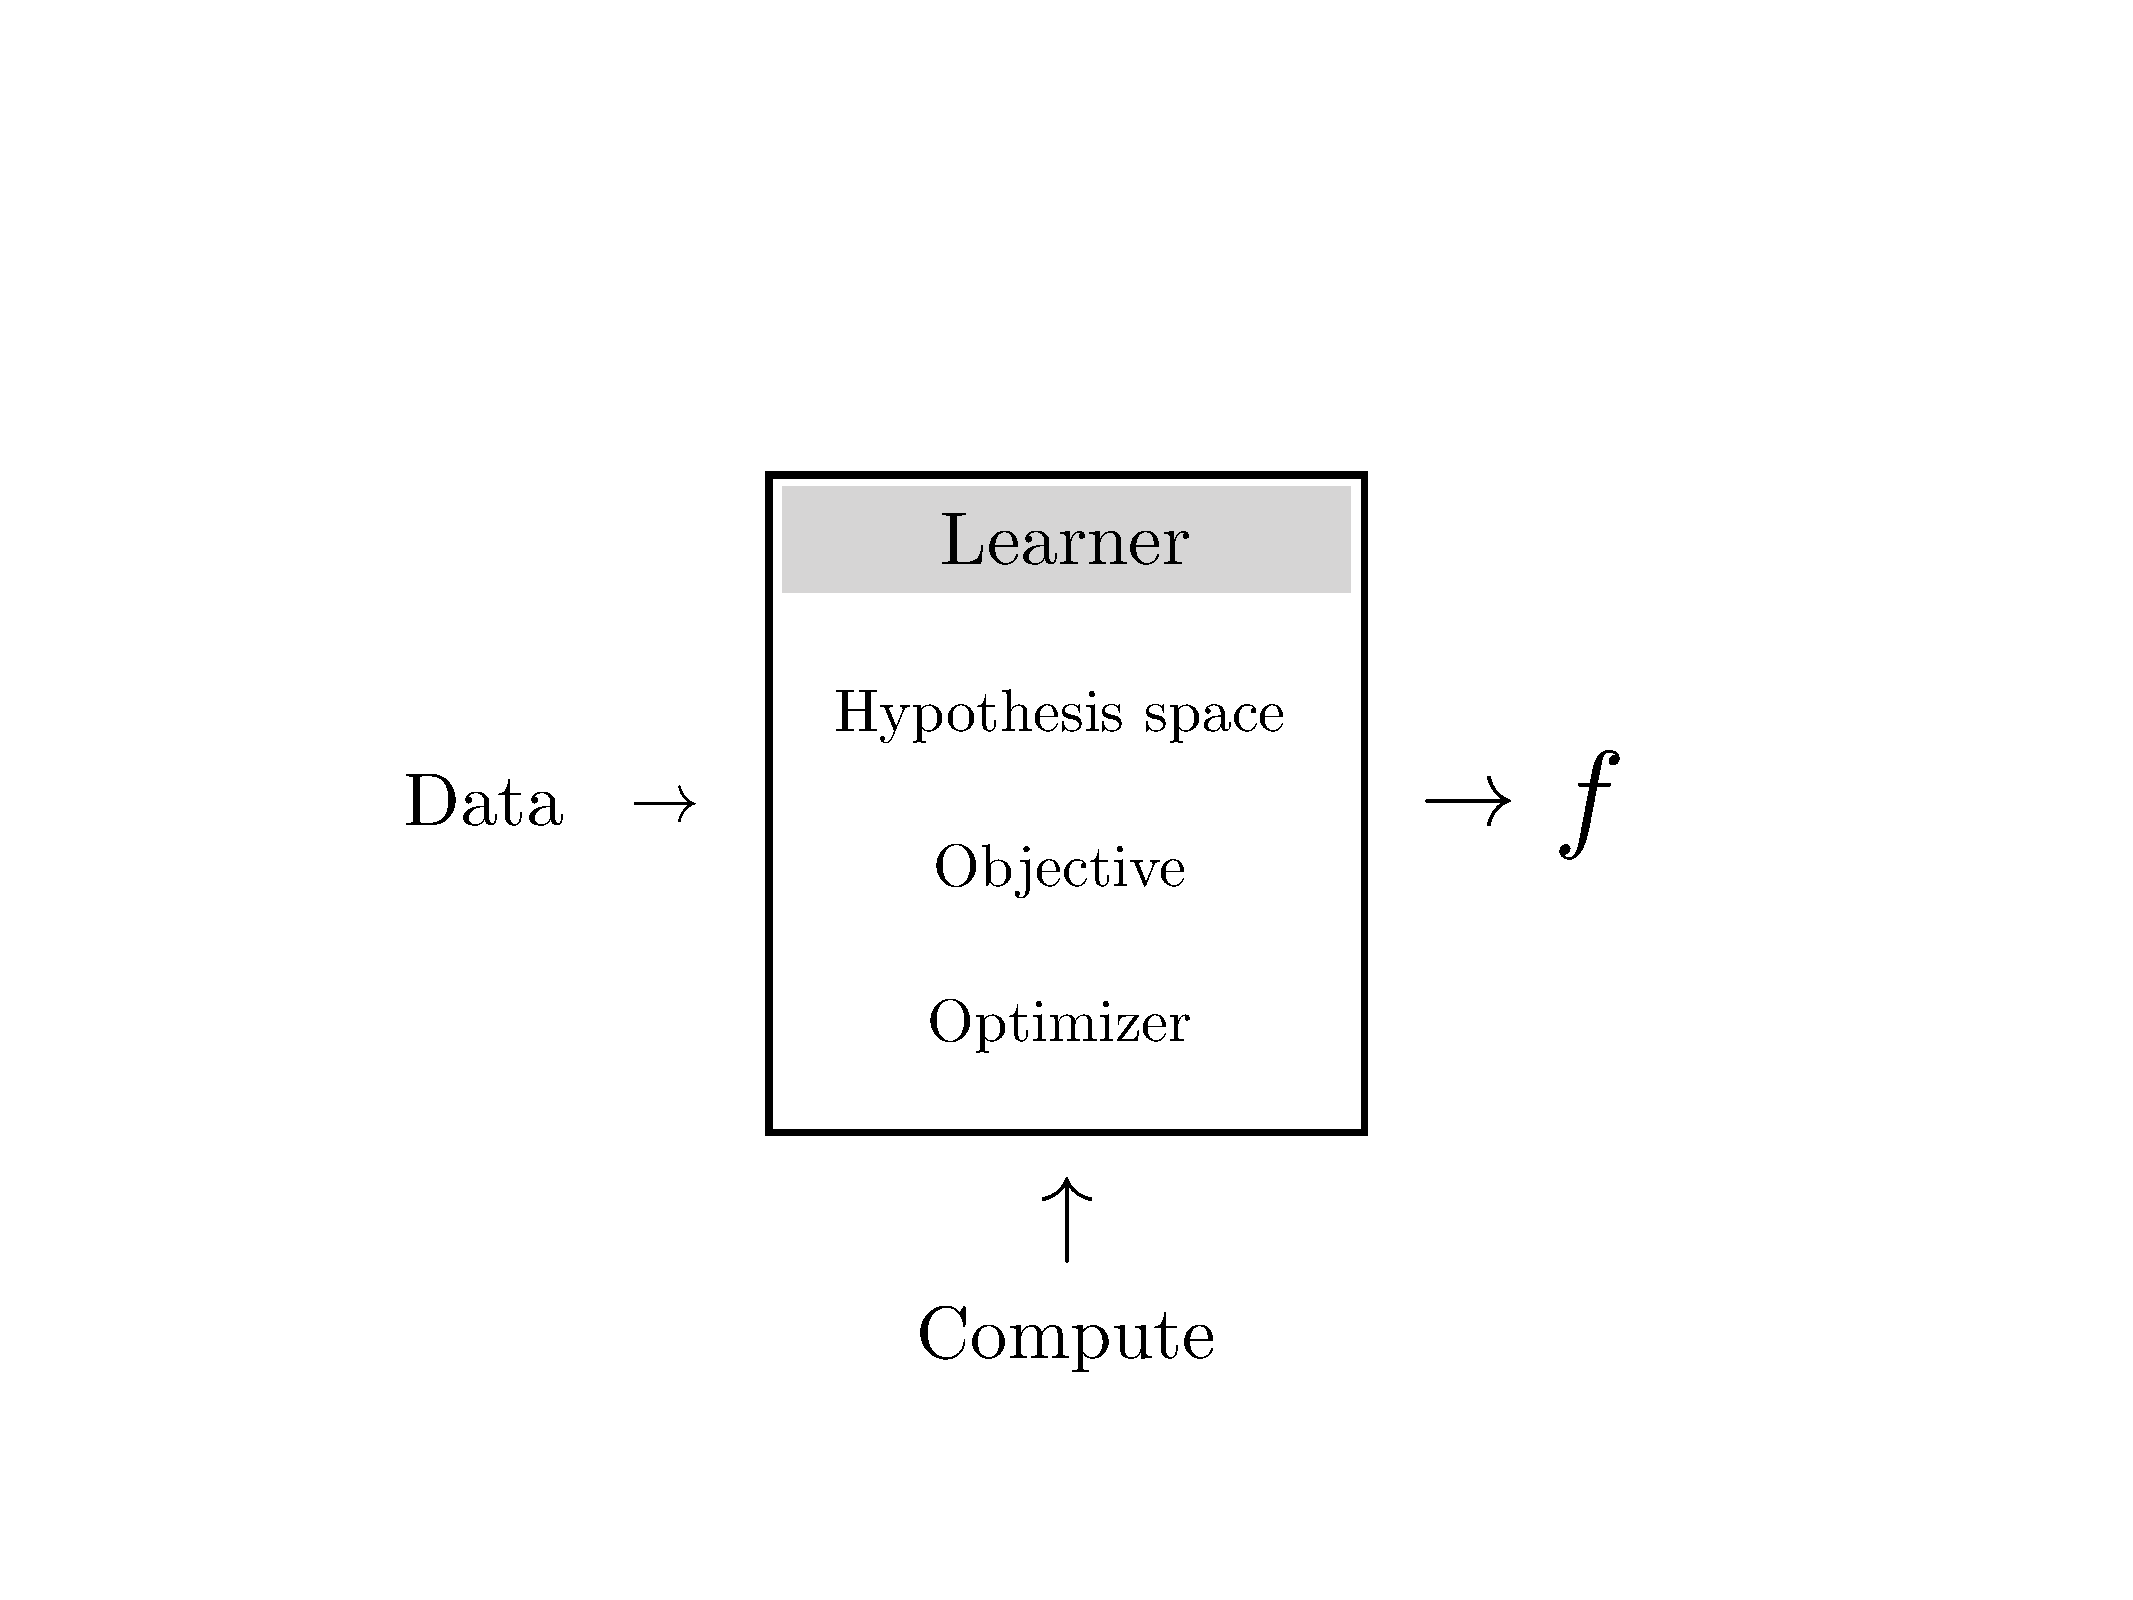
\includegraphics[width=0.5\linewidth]{./figures/intro_to_learning/ingredients.pdf}
%     \label{fig:ingredients}
% \end{figure}

A learner outputs an algorithm, $f: \mathcal{X} \rightarrow \mathcal{Y}$, which maps inputs, $\mathbf{x} \in \mathcal{X}$, to outputs, $\mathbf{y} \in \mathcal{Y}$. Commonly, $f$ is referred to as the \index{Learned function}\textbf{learned function}. The objective that the learner optimizes is typically a function that scores model outputs, $\mathcal{L}: \mathcal{Y} \rightarrow \mathbb{R}$, or compares model outputs to target answers, $\mathcal{L}: \mathcal{Y} \times \mathcal{Y} \rightarrow \mathbb{R}$. We will interchangeably call this $\mathcal{L}$ either the \textbf{objective function}, the \index{Loss function}\textbf{loss function}, or the \textbf{loss}. A loss almost always refers to an objective we seek to \textit{minimize}, whereas an objective function can be used to describe objectives we seek to minimize as well as those we seek to maximize.

\subsection{Importance of Parameterization} The hypothesis space can be described by a set $\mathcal{F}$ of all the possible functions under consideration by the learner. For example, one hypothesis space might be ``all mappings from $\mathbb{R}^2 \rightarrow \mathbb{R}$'' and another could be ``all functions $\mathbb{R} \times \mathbb{R} \rightarrow \mathbb{R}_{\geq 0}$ that satisfy the conditions of being a distance metric.'' Commonly, however, we will not just specify the hypothesis space, but also how we parameterize the space. For example, we may say that our \textit{parameterized} hypothesis space is $y = \theta_1 x + \theta_0$, where $\theta_0$ and $\theta_1$ are the parameters. This example corresponds to the space of affine functions from $\mathbb{R} \rightarrow \mathbb{R}$, but this is not the only way to parameterize that space. Another choice could be $y = \theta_2\theta_1 x + \theta_0$, with parameters $\theta_0$, $\theta_1$, and $\theta_2$. These two choices parameterize \textit{exactly the same space}, that is, any affine functions can be represented by either parameterization and both parameterizations can only represent affine functions. However, these two parameterizations are not equivalent, because optimizers and objectives may treat different parameterizations differently. Because of this, to fully define a learning algorithm, it is important to specify how the hypothesis space is parameterized.\marginnote{\index{Overparameterization}\textbf{Overparameterized} models, where you use more parameters than the minimum necessary to fit the data, are especially important in modern computer vision; most neural networks (\chap{\ref{chapter:neural_nets}}) are overparameterized.}[-3.4cm]
%\marginnote{Recall that a metric function is a very constrained class of functions; metrics must satisfy the triangle inequality, symmetry, nonnegativity, and ``identity of indiscernibles."}
%\marginnote{The role of parameterization can be subtle but should not be overlooked. Historically ... }

\section{Empirical Risk Minimization: A Formalization of Learning from Examples}

The three ingredients from the last section can be formalized using the framework of \index{Empirical risk minimization}{\bf empirical risk minimization} ({\bf ERM}). This framework applies specifically to the supervised setting where we are learning a function that predicts $\mathbf{y}$ from $\mathbf{x}$ given many training examples $\{\mathbf{x}^{(i)},\mathbf{y}^{(i)}\}^N_{i=1}$. The idea is to minimize the average error (i.e., risk) we incur over all the training data (i.e., empirical distribution). The ERM problem is stated as follows:
\begin{align}
    \argmin_{f \in \mathcal{F}} \frac{1}{N} \sum_{i=1}^N \mathcal{L}(f(\mathbf{x}^{(i)}),\mathbf{y}^{(i)}) \quad\triangleleft\quad \text{ERM}
\end{align}
Here, $\mathcal{F}$ is the hypothesis space, $\mathcal{L}$ is the loss function, and $\{\mathbf{x}^{(i)}, \mathbf{y}^{(i)}\}_{i=1}^N$ is the training data (example \{\texttt{input}, \texttt{output}\} pairs), and $f$ is the learned function.

\section{Learning as Probabilistic Inference}
Depending on the loss function, there is often an interpretation of ERM as doing maximum likelihood probabilistic inference. In this interpretation, we are trying to infer the hypothesis $f$ that assigns the highest probability to the data. For a model that predicts $\mathbf{y}$ given $\mathbf{x}$, the max likelihood $f$ is:
\begin{align}
    \argmax_f p\big(\{\mathbf{y}^{(i)}\}_{i=1}^N \given \{\mathbf{x}^{(i)}\}_{i=1}^N, f\big) \quad\quad \triangleleft \quad\text{Max likelihood learning}
\end{align}
The term $p\big(\{\mathbf{y}^{(i)}\}_{i=1}^N \given \{\mathbf{x}^{(i)}\}_{i=1}^N, f\big)$ is called the \index{Likelihood}\textbf{likelihood} of the $\mathbf{y}$ values given the model $f$ and the observed $\mathbf{x}$ values, and maximizing this quantity is called \index{Maximum likelihood learning}\textbf{maximum likelihood learning}.\marginnote{To fully specify this model, we have to define the form of this conditional distribution. One common choice is that the prediction errors, $(\mathbf{y} - f(\mathbf{x}))$, are Gaussian distributed, which leads to the least-squares objective (\sect{\ref{sec:intro_to_learning:least_squares}}).}[-0.4cm]

In later chapters we will see that \textbf{priors} $p(f)$ can also be used for inferring the most probable hypothesis. When a prior is used in conjunction with a likelihood function, we arrive at \index{Maximum a posteriori learning}\textbf{maximum a posteriori learning} (\textbf{MAP learning}), which infers the most probable hypothesis given the training data:
\begin{align}
    &\argmax_f p\big(f \given \{\mathbf{x}^{(i)}, \mathbf{y}^{(i)}\}_{i=1}^N\big) \quad\quad \triangleleft \quad \text{MAP learning}\\
    & = \argmax_f p\big(\{\mathbf{y}^{(i)}\}_{i=1}^N \given \{\mathbf{x}^{(i)}\}_{i=1}^N, f\big)p\big(f\big) \quad\quad \triangleleft \quad \text{by Bayes' rule}
\end{align}


%For example, the least squares regression example we saw above can be interpreted as finding the maximum likelihood estimate of the parameters $\theta$ given the assumption that there truly exists a linear relationship between $x$ and $y$ but that training observations of $y$ are corrupted by Gaussian noise (and we assume that training datapoints are independent and identically distributed, i.e. {\bf iid}).





\section{Case Studies}
The next three sections cover several case studies of particular learning problems. Examples 1 and 3 showcase the two most common workhorses of machine learning: regression and classification. Example 2, Python program induction, demonstrates that the paradigms in this chapter are not limited to simple systems but can actually apply to very general and sophisticated models.

\subsection{Example 1: Linear Least-Squares Regression}\label{sec:intro_to_learning:least_squares}
One of the simplest learning problems is known as \index{Linear least-squares regression}\textbf{linear least-squares regression}. In this setting, we aim to model the relationship between two variables, $x$ and $y$, with a line. 

As a concrete example, let's imagine $x$ represents the temperature outside, and $y$ represents the number people at the beach. As before, we train (i.e., fit) our model on many observed examples of \{\texttt{temperature outside}, \texttt{number of people at the beach}\} pairs, denoted as $\{x^{(i)},y^{(i)}\}_{i=1}^N$. At test time, this model can be applied to predict the $y$ value of a new query $x'$, as shown in \fig{\ref{fig:intro_to_learning:ols_train_test}}.

\begin{figure}[h]
    \centerline{
    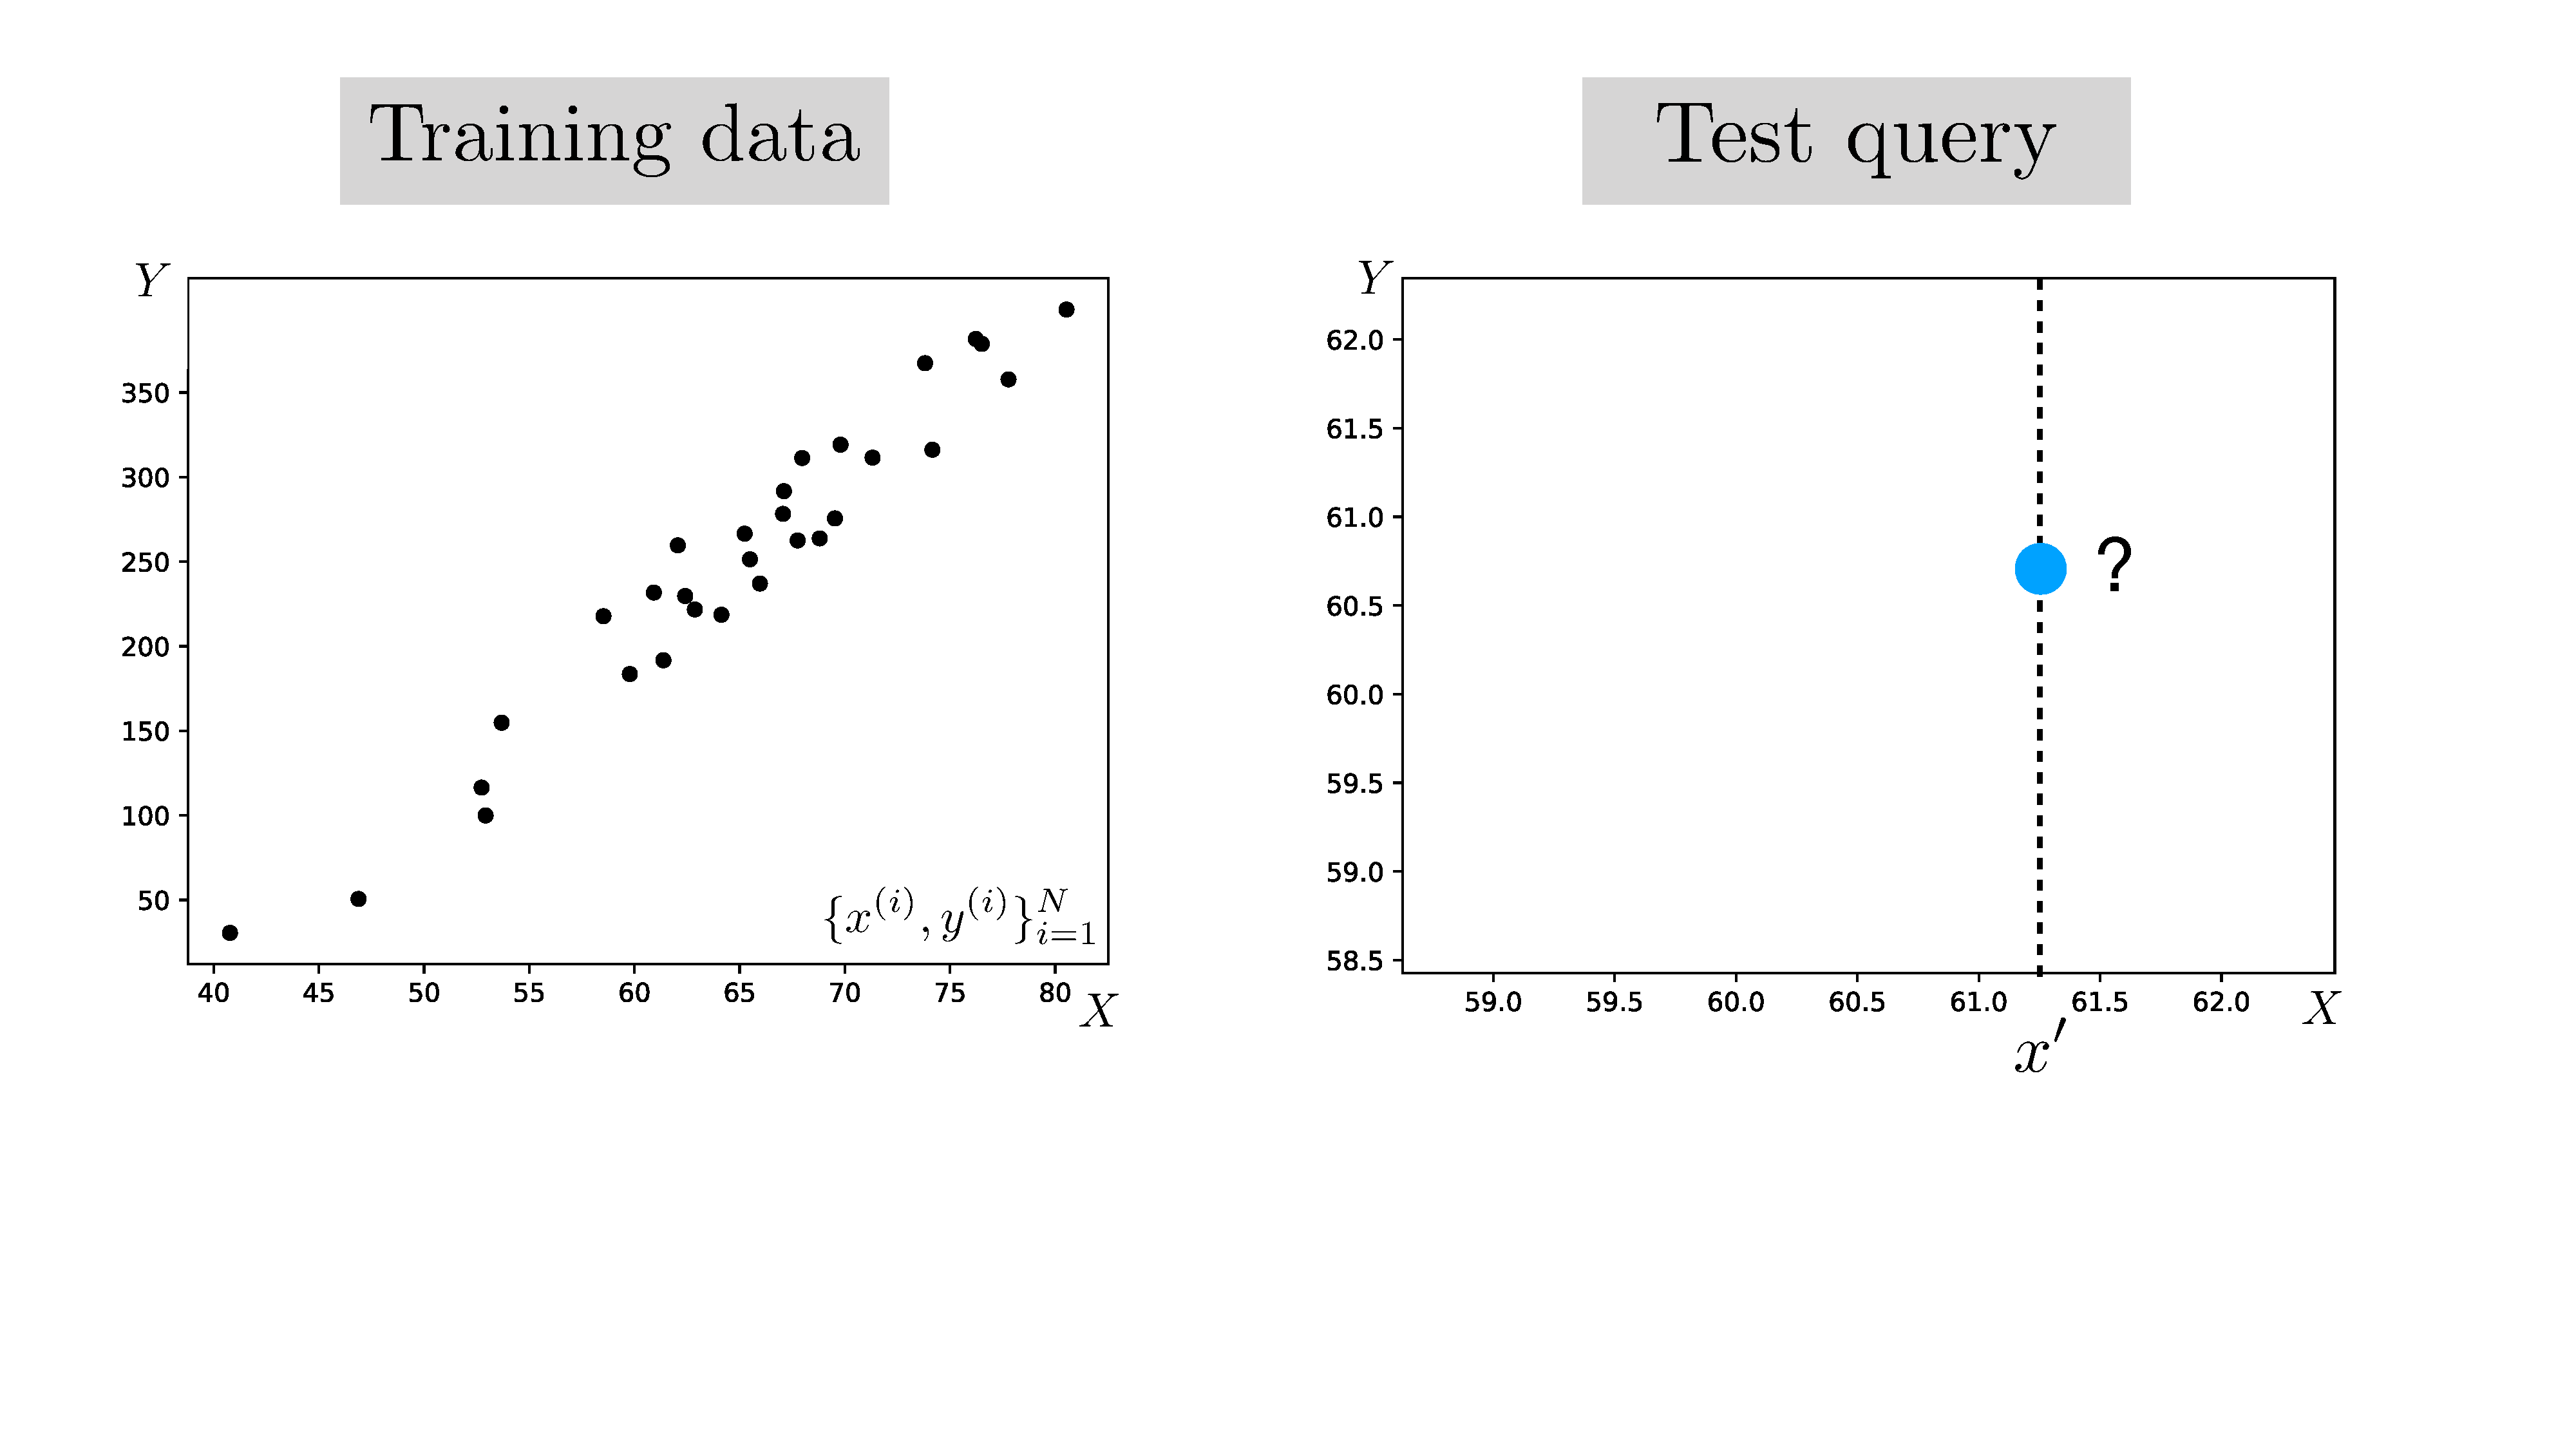
\includegraphics[width=0.7\linewidth]{./figures/intro_to_learning/ols_train_test.pdf}
    }
    \caption{The goal of learning is to use the training data to predict the $y$ value of the test query. In our example we find that for every 1 degree increase in temperature, we can expect $\sim 10$ more people to go to the beach.}
    \label{fig:intro_to_learning:ols_train_test}
\end{figure}

Our \emph{hypothesis space} is linear functions, that is, the relationship between $x$ and our predictions $\hat{y}$ of $y$ has the form $\hat{y} = f_{\theta}(x) = \theta_1 x + \theta_0$. This hypothesis space is parameterized by a two scalars, $\theta_0, \theta_1 \in \mathbb{R}$, the intercept and slope of the line. In this book, we will use $\theta$ in general to refer to any parameters that are being learned. In this case we have $\theta = [\theta_0, \theta_1]$. Learning consists of finding the value of these parameters that maximizes the objective.

Our \emph{objective} is that predictions should be near ground truth targets in a least-squares sense, that is, $(\hat{y}^{(i)} - y^{(i)})^2$ should be small for all training examples $\{x^{(i)}, y^{(i)}\}_{i=1}^N$. We call this objective the $L_2$ loss:
\begin{align}
    J(\theta) &= \sum_i \mathcal{L}(\hat{y}^{(i)}, y^{(i)})\\
    &\quad \mathcal{L}(\hat{y}, y) = (\hat{y} - y)^2 \quad\quad \triangleleft \quad L_2 \text{ loss}
\end{align}
\marginnote{We will use $J(\theta)$ to denote the total objective, over all training datapoints, as a function of the parameters; we will use $\mathcal{L}$ to denote the loss per datapoint. That is, $J(\theta) = \sum_{i=1}^N \mathcal{L}(f_{\theta}(x^{(i)}), y^{(i)})$.}[-1.5cm]%Some texts refer to $J$, rather than $\mathcal{L}$, as the ``loss function", but we will reserve the distinct term ``total cost" for $J$ and ``loss" for $\mathcal{L}$.}

%$\mathcal{L}(\hat{y},y) = (\hat{y} - y)^2$ is referred to as the {\bf loss function}, which is defined as the negative of the objective.
%\marginnote{Minimizing the {\bf loss} is equivalent to maximizing the objective.}[-0.0cm]

The full learning problem is as follows:
\begin{align}
    \theta^* = \argmin_{\theta} \sum_{i=1}^N (\theta_1 x^{(i)} + \theta_0 - y^{(i)})^2.
\end{align}
We can choose any number of optimizers to solve this problem. A first idea might be ``try a bunch of random values for $\theta$ and return the one that maximizes the objective.'' In fact, this simple approach works, it just can be rather slow since we are searching for good solutions blind. A better idea can be to exploit \textit{structure} in the search problem. For the linear least-squares problem, the tools of calculus give us clean mathematical structure that makes solving the optimization problem easy, as we show next.

From calculus, we know that at any maxima or minima of a function, $J(\theta)$, with respect to a variable $\theta$, the derivative $\frac{\partial{J(\theta)}}{\partial{\theta}} = 0$. We are trying to find the minimum of the objective $J(\theta)$:
\begin{align}
    J(\theta) = \sum_{i=1}^N (\theta_1 x^{(i)} + \theta_0 - y^{(i)})^2.
\end{align}
This function can be rewritten as
\begin{align}
    J(\theta) = (\mathbf{y} - \mathbf{X}\theta)^\transpose(\mathbf{y} - \mathbf{X}\theta)
\end{align}
with
\begin{align}
\mathbf{X} = 
 \begin{bmatrix}
    1 & x^{(1)}  \\
    1 & x^{(2)} \\
    \vdots & \vdots \\
    1 & x^{(N)}
\end{bmatrix}
\quad
\mathbf{y} = 
 \begin{bmatrix}
    y^{(1)}  \\
    y^{(2)} \\
    \vdots \\
    y^{(N)}
\end{bmatrix}
\quad
\theta = 
 \begin{bmatrix}
    \theta_0 \\
    \theta_1
\end{bmatrix}.
\end{align}

The $J$ is a quadratic form, which has a single global minimum where the derivative is zero, and no other points where the derivative is zero. Therefore, we can solve for the $\theta^*$ that minimizes $J$ by finding the point where the derivative is zero. The derivative is:
\begin{align}
    \frac{\partial J(\theta)}{\partial \theta} =  2(\mathbf{X}^\transpose \mathbf{X} \theta - \mathbf{X}^\transpose \mathbf{y}).
\end{align}
We set this derivative to zero and solve for $\theta^*$:
\begin{align}
    2(\mathbf{X}^\transpose \mathbf{X} \theta^* - \mathbf{X}^\transpose \mathbf{y}) &= 0\\
\mathbf{X}^\transpose \mathbf{X} \theta^* &= \mathbf{X}^\transpose \mathbf{y}\\
\theta^* &= (\mathbf{X}^\transpose\mathbf{X})^{-1}\mathbf{X}^\transpose\mathbf{y}.
\end{align}

The $\theta^*$ defines the best fitting line to our data, and this line can be used to predict the $y$ value of future observations of $x$ (\fig{\ref{fig:intro_to_learning:ols_fit}}).

\begin{figure}[h]
    \centerline{
    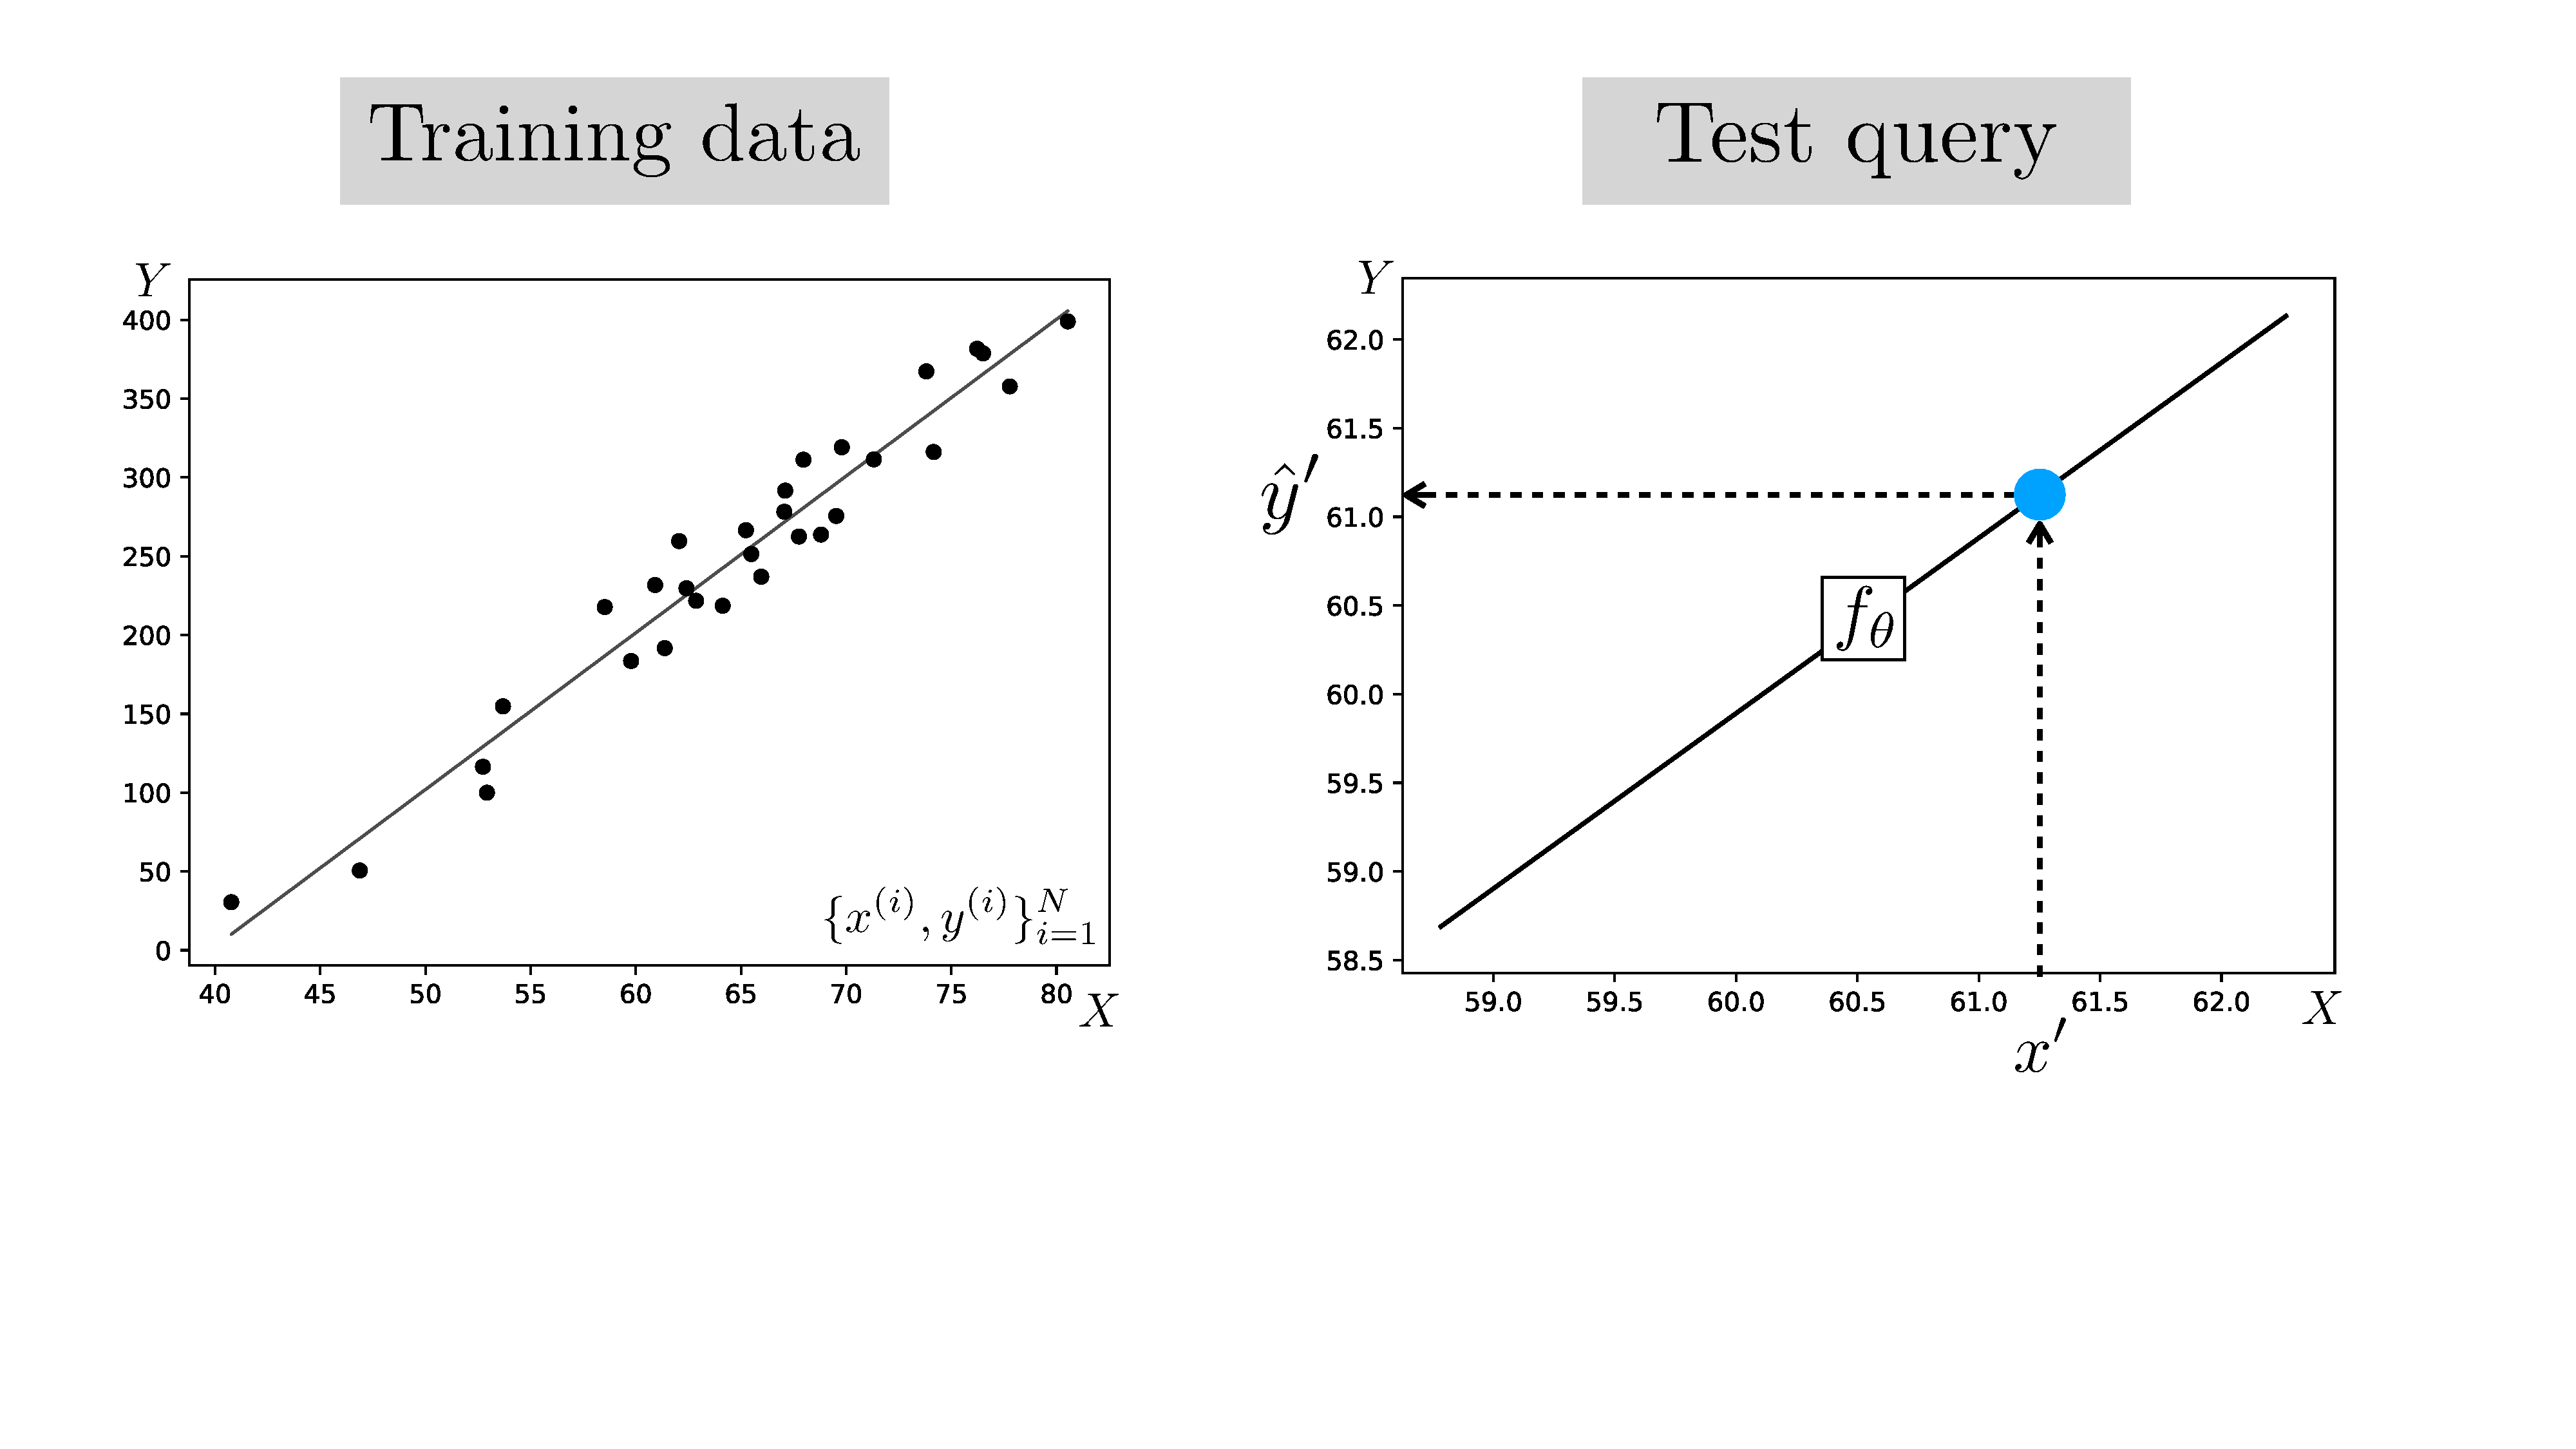
\includegraphics[width=1\linewidth]{./figures/intro_to_learning/ols_fit.pdf}
    }
    \caption{A best fit line is a visualization of a function $f_{\theta}$, that predicts the $y$-value for each input $x$-value.}
    \label{fig:intro_to_learning:ols_fit}
\end{figure}

We can now summarize the entire linear least-squares learning problem as follows:

\begin{center}
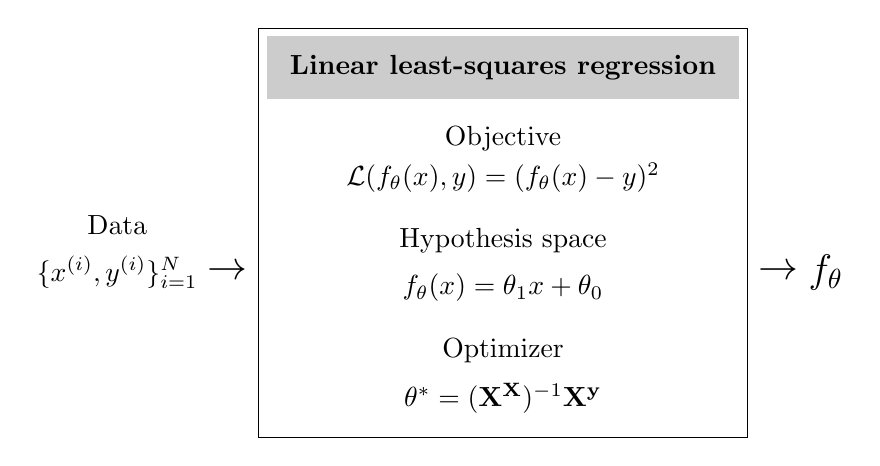
\begin{tikzpicture}
    \draw (0,0) rectangle (6.2,5.2); % outer box
    \fill[black!20] (0.1,4.3) rectangle (6.1,5.1); % gray box
    \node[] at (3.1,4.7) {{\bf Linear least-squares regression}};
    \node[] at (3.1,3.8) {Objective}; \node[] at (3.1,3.3) {$\mathcal{L}(f_{\theta}(x),y) = (f_{\theta}(x)-y)^2$};
    \node[] at (3.1,2.5) {Hypothesis space}; \node[] at (3.1,1.9) {$f_{\theta}(x) = \theta_1 x + \theta_0$};
    \node[] at (3.1,1.1) {Optimizer}; \node[] at (3.1,0.5) {$\theta^* = (\mathbf{X}^\transpose\mathbf{X})^{-1}\mathbf{X}^\transpose\mathbf{y}$};
    \node[] at (-1.8,2.7) {Data};
    \node[] at (-1.8,2.1) {$\{x^{(i)}, y^{(i)}\}_{i=1}^N$};
    \node[] at (-0.4,2.1) {{\Large  $ \rightarrow$}};
    \node[] at (7.2,2.1) {{\Large $f_{\theta}$}};
    \node[] at (6.6,2.1) {{\Large  $ \rightarrow$}};
\label{fig:ols_summary}
\end{tikzpicture}
\end{center}
% \begin{figure}[h]
%     \centering
%     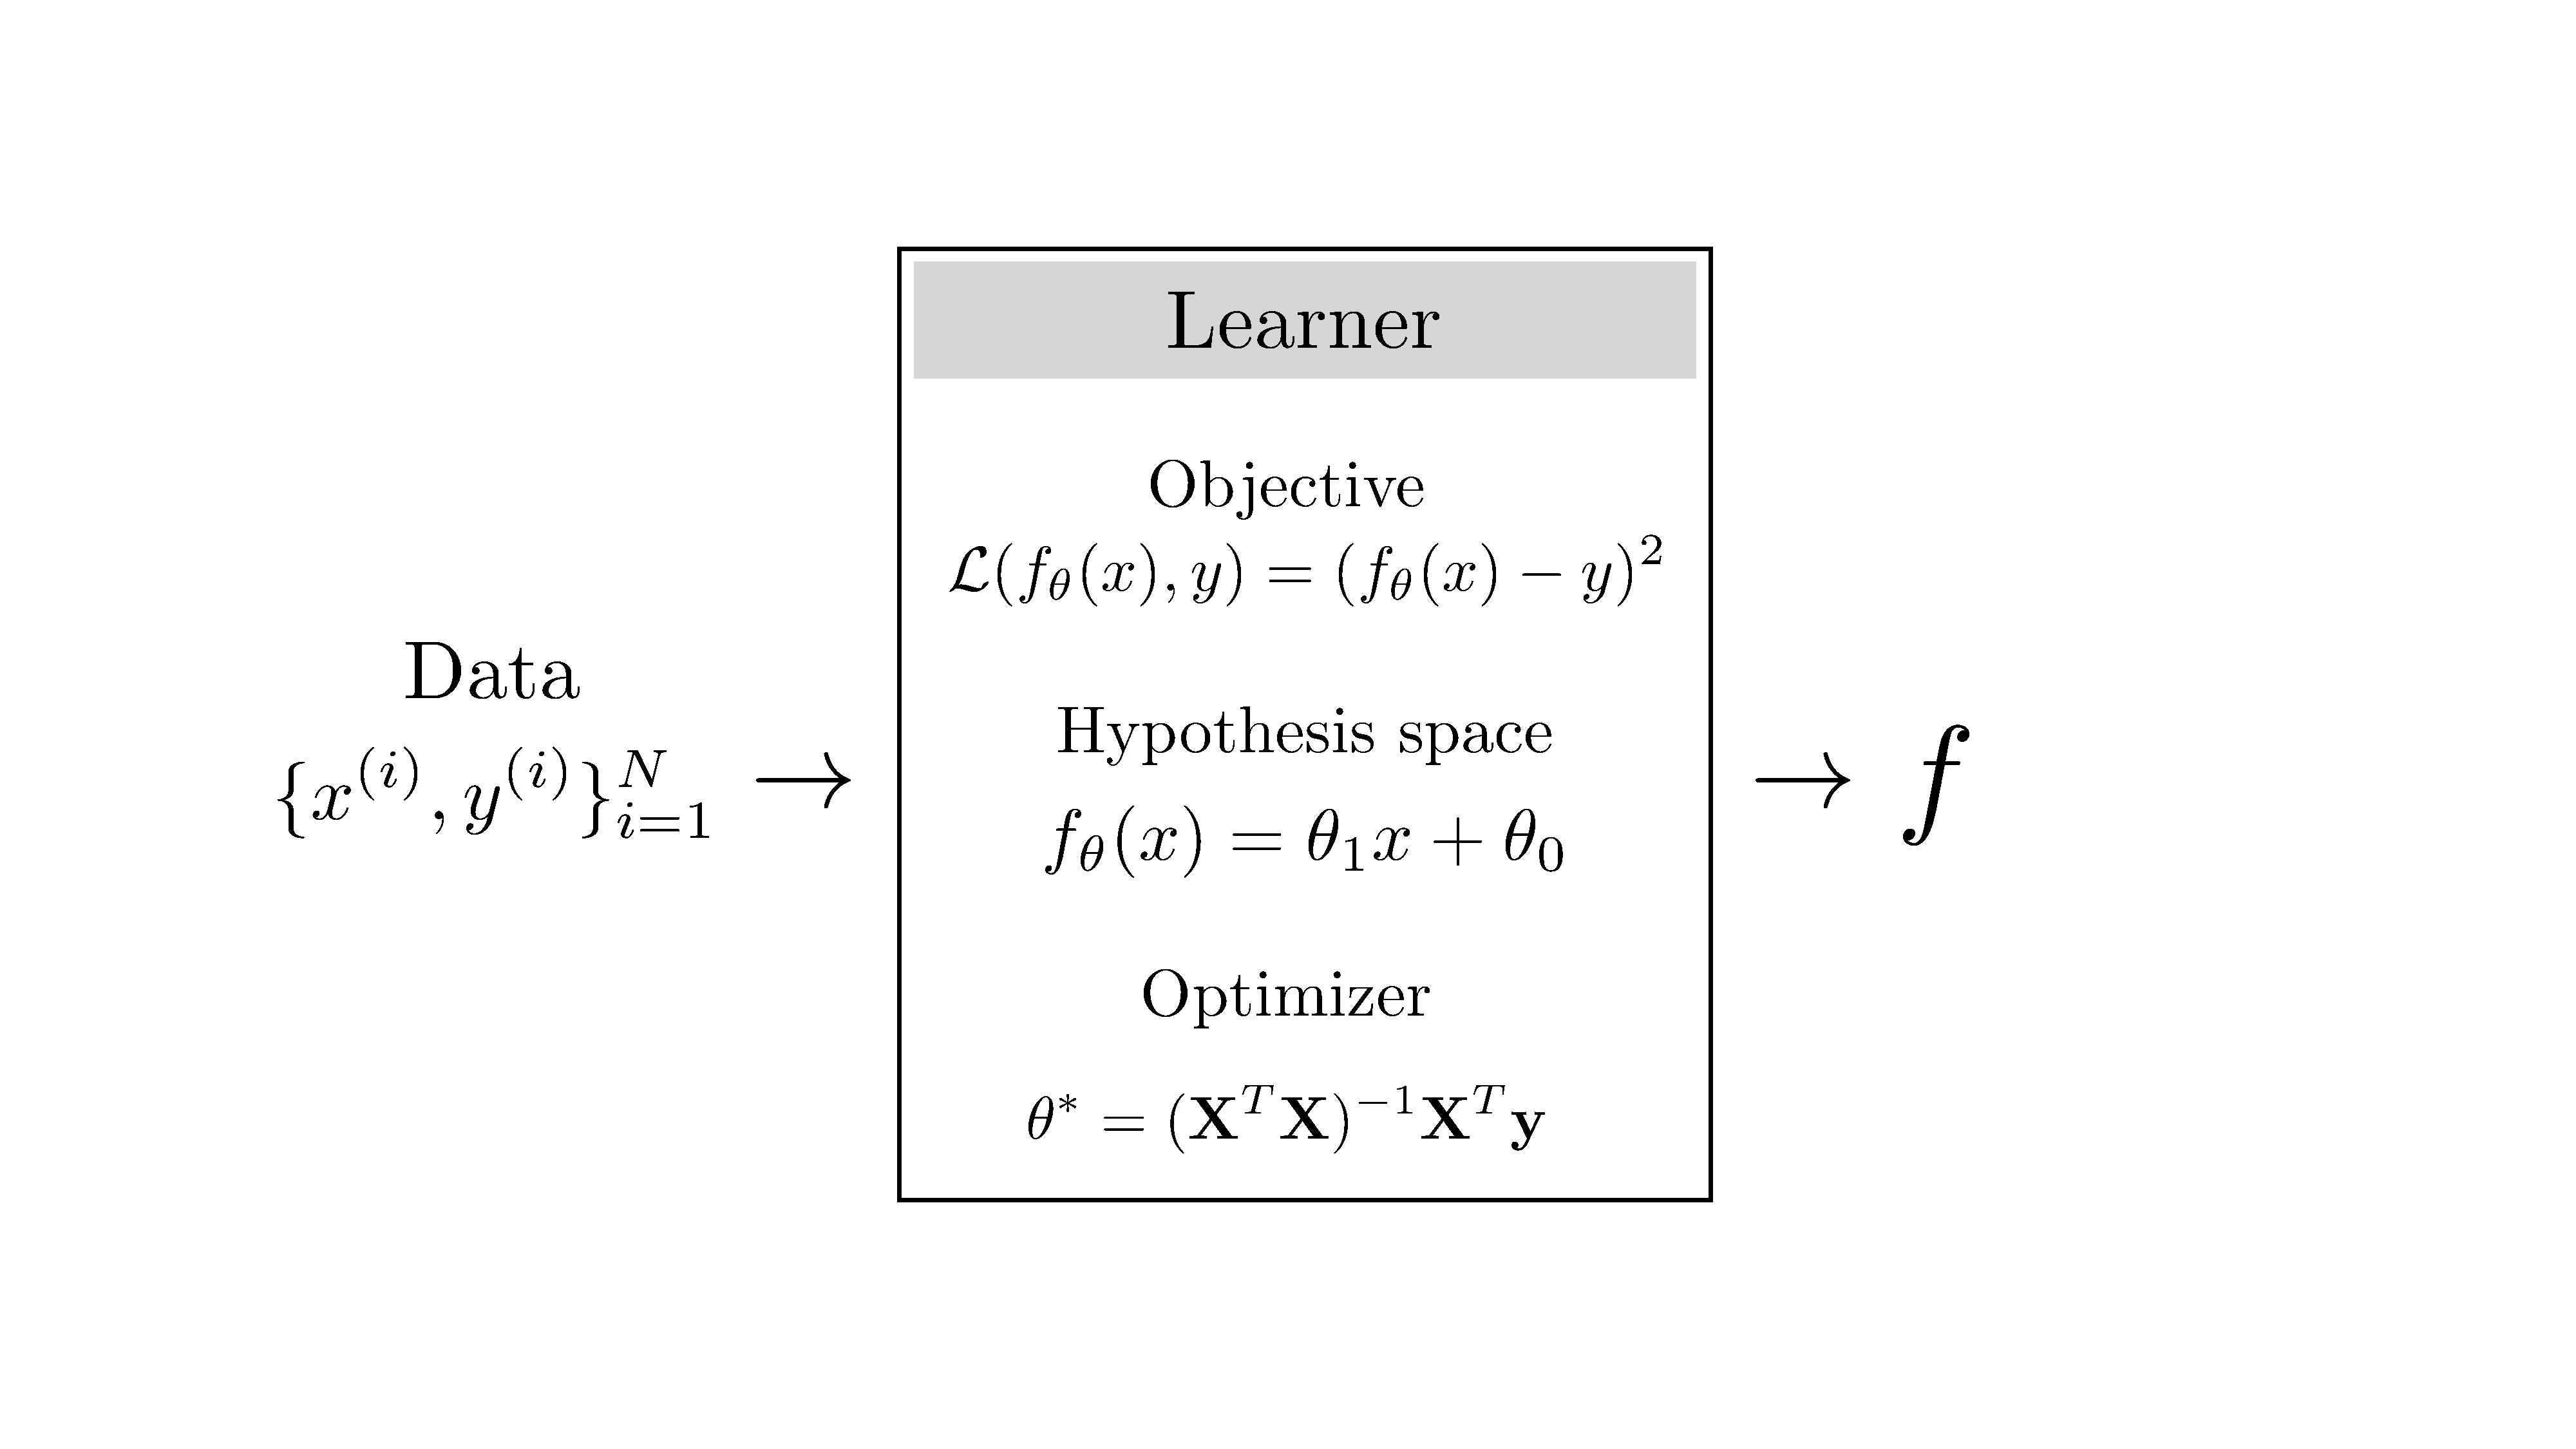
\includegraphics[width=0.6\linewidth]{./figures/intro_to_learning/ols_summary.pdf}
%     \label{fig:ols_summary}
% \end{figure}
\marginnote{In these diagrams, we will sometimes describe the objective just in terms of $\mathcal{L}$, in which case it should be understood that this implies $J(\theta) = \sum_{i=1}^N \mathcal{L}(f_{\theta}(x^{(i)}), y^{(i)})$.}[-4cm]

\subsection{Example 2: Program Induction}
At the other end of the spectrum we have what is known as \index{Program induction}\textbf{program induction}, which is one of the broadest classes of learning algorithm. In this setting, our hypothesis space may be all Python programs. Let's contrast linear least-squares with Python program induction. \Fig{\ref{fig:intro_to_learning:ols_system_diagram}} shows what linear least-squares looks like.

\begin{figure}[h]
    \centerline{
    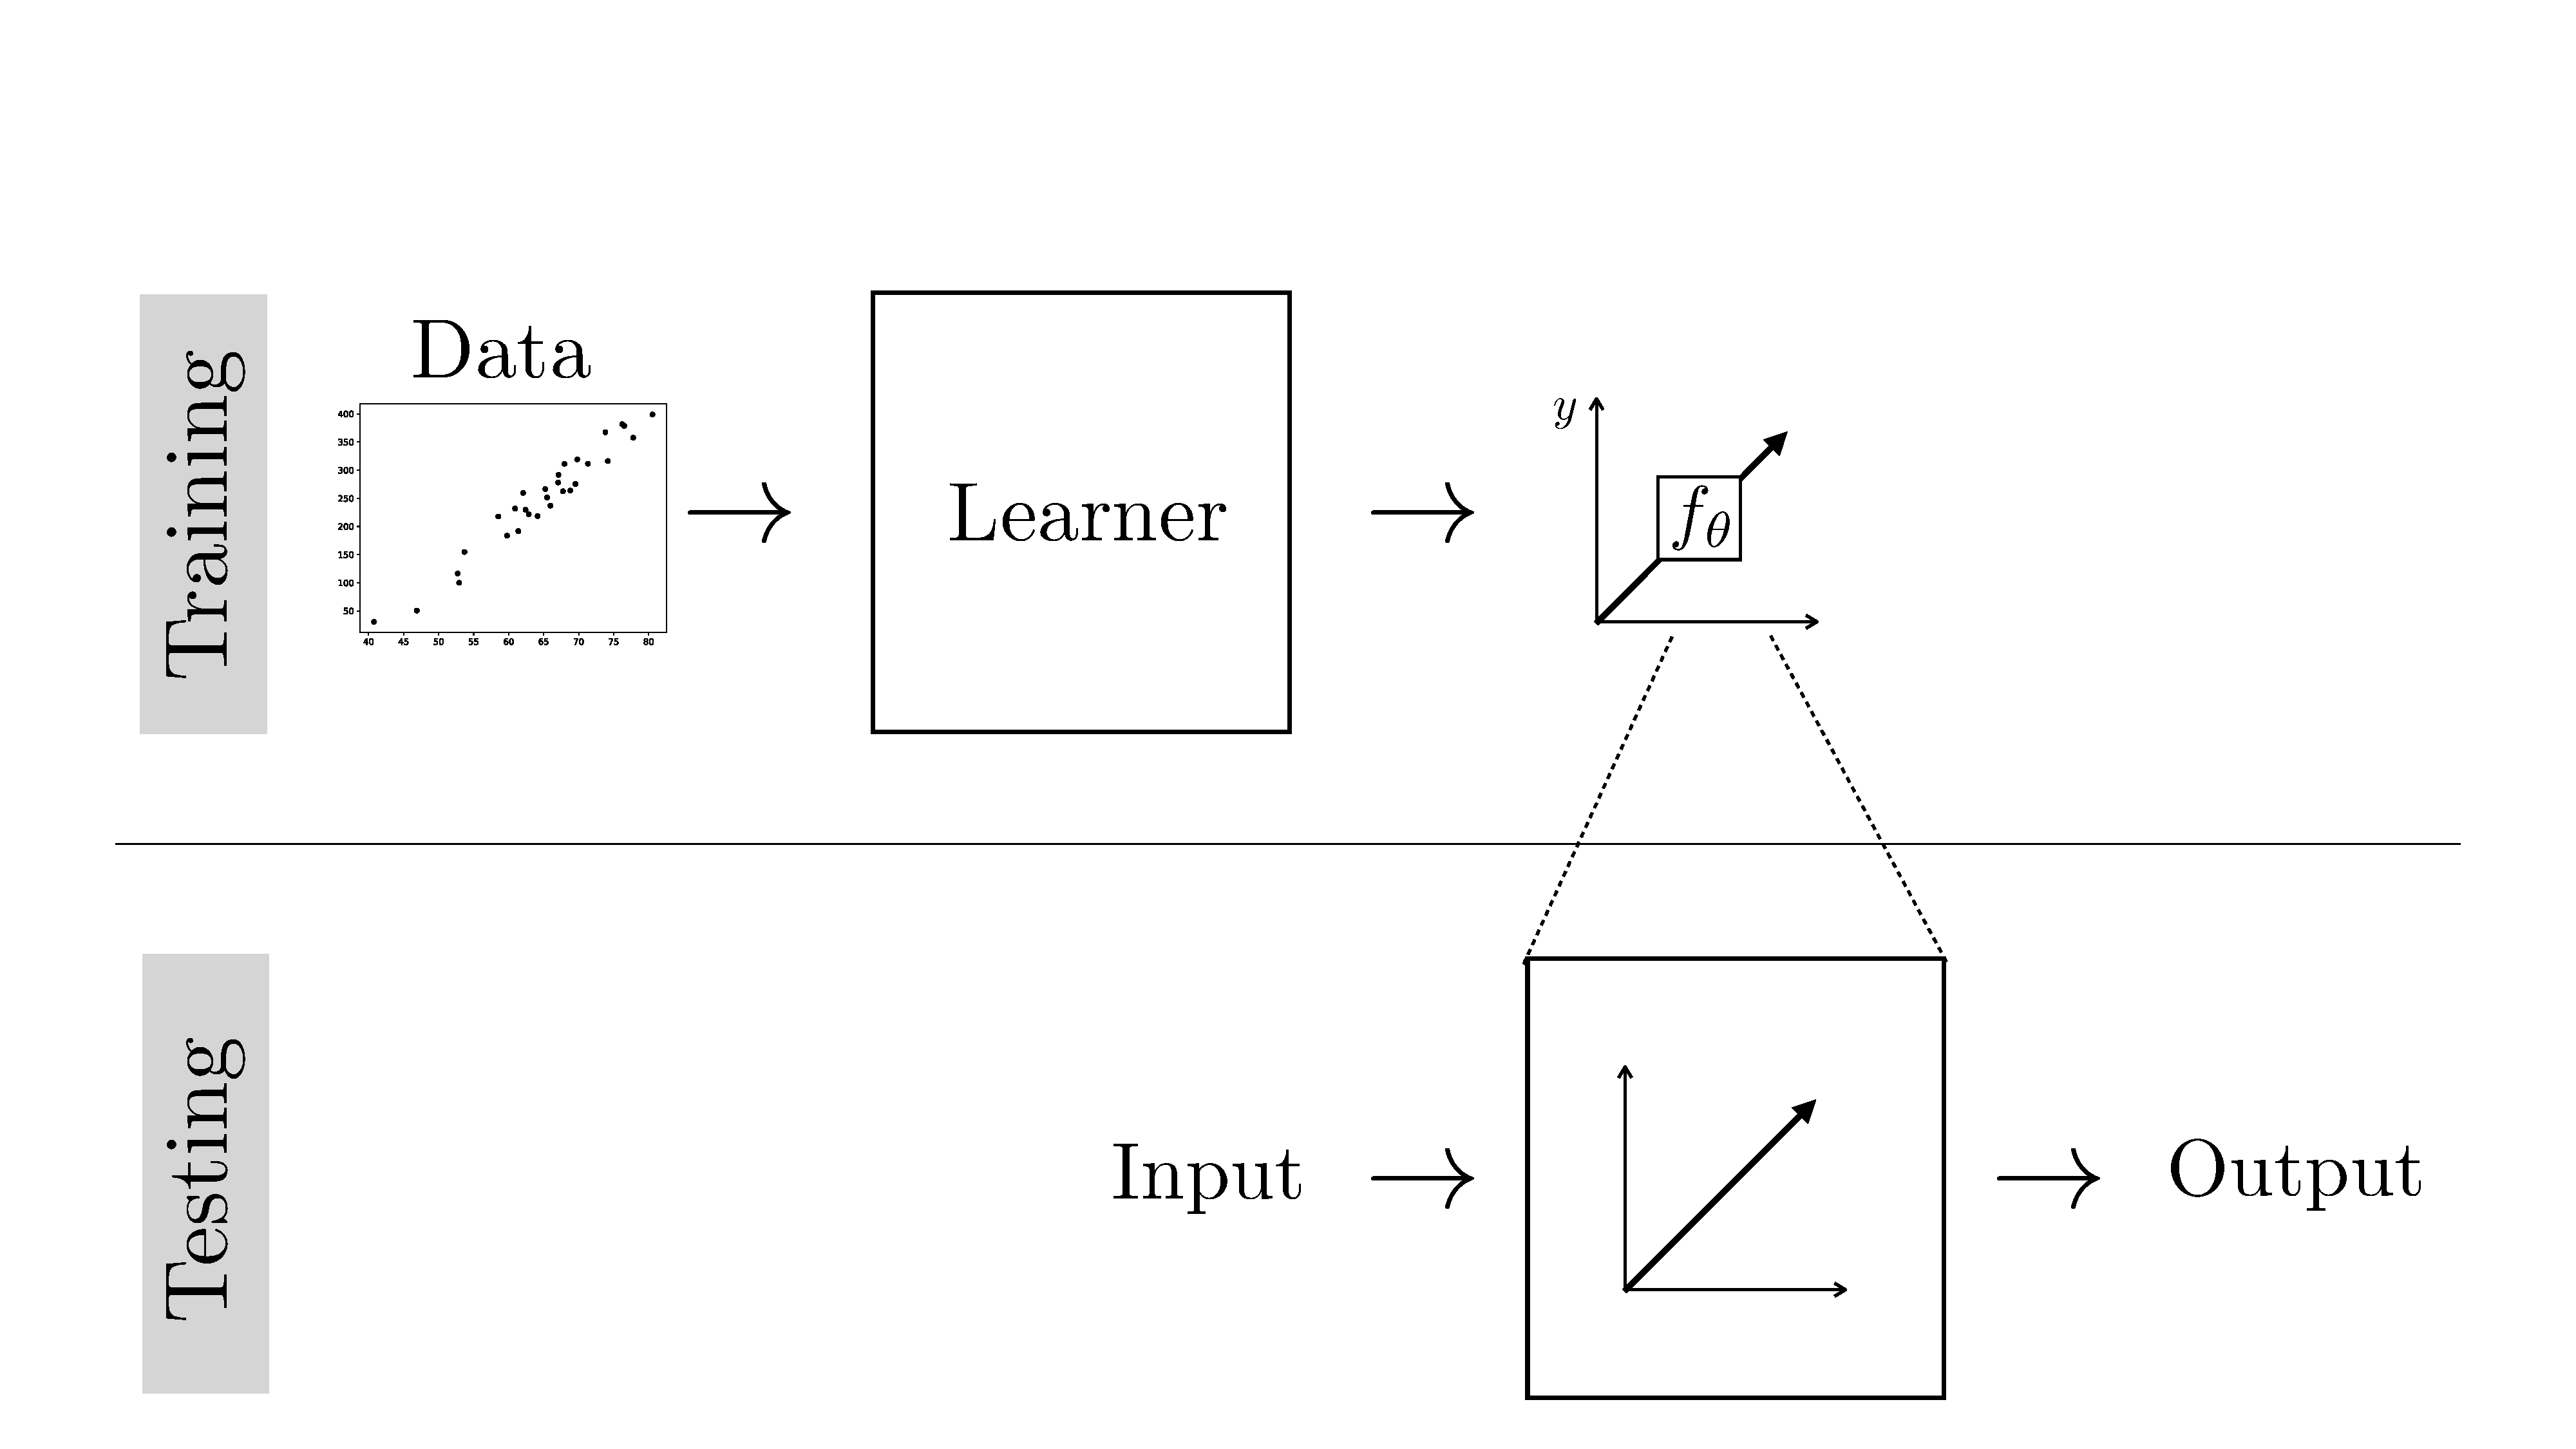
\includegraphics[width=0.8\linewidth]{./figures/intro_to_learning/ols_system_diagram.pdf}
    }
    \caption{Linear regression finds a line that predicts the training data's $y$-values from its $x$-values.}
    \label{fig:intro_to_learning:ols_system_diagram}
\end{figure}

The learned function is an algebraic expression that maps $x$ to $y$. Learning consisting of searching over two scalar parameters, $\theta_0$ and $\theta_1$.

\Fig{\ref{fig:intro_to_learning:program_induction_system_diagram}} shows Python program induction solving the same problem. In this case, the learned function is a Python program that maps $x$ to $y$. Learning consisted of searching over the space of all possible Python programs (within some max length). Clearly that's a much harder search problem than just finding two scalars. In \chap{\ref{chapter:problem_of_generalization}}, we will see some pitfalls of using too powerful a hypothesis space when a simpler one will do.

\begin{figure}[h]
    \centerline{
    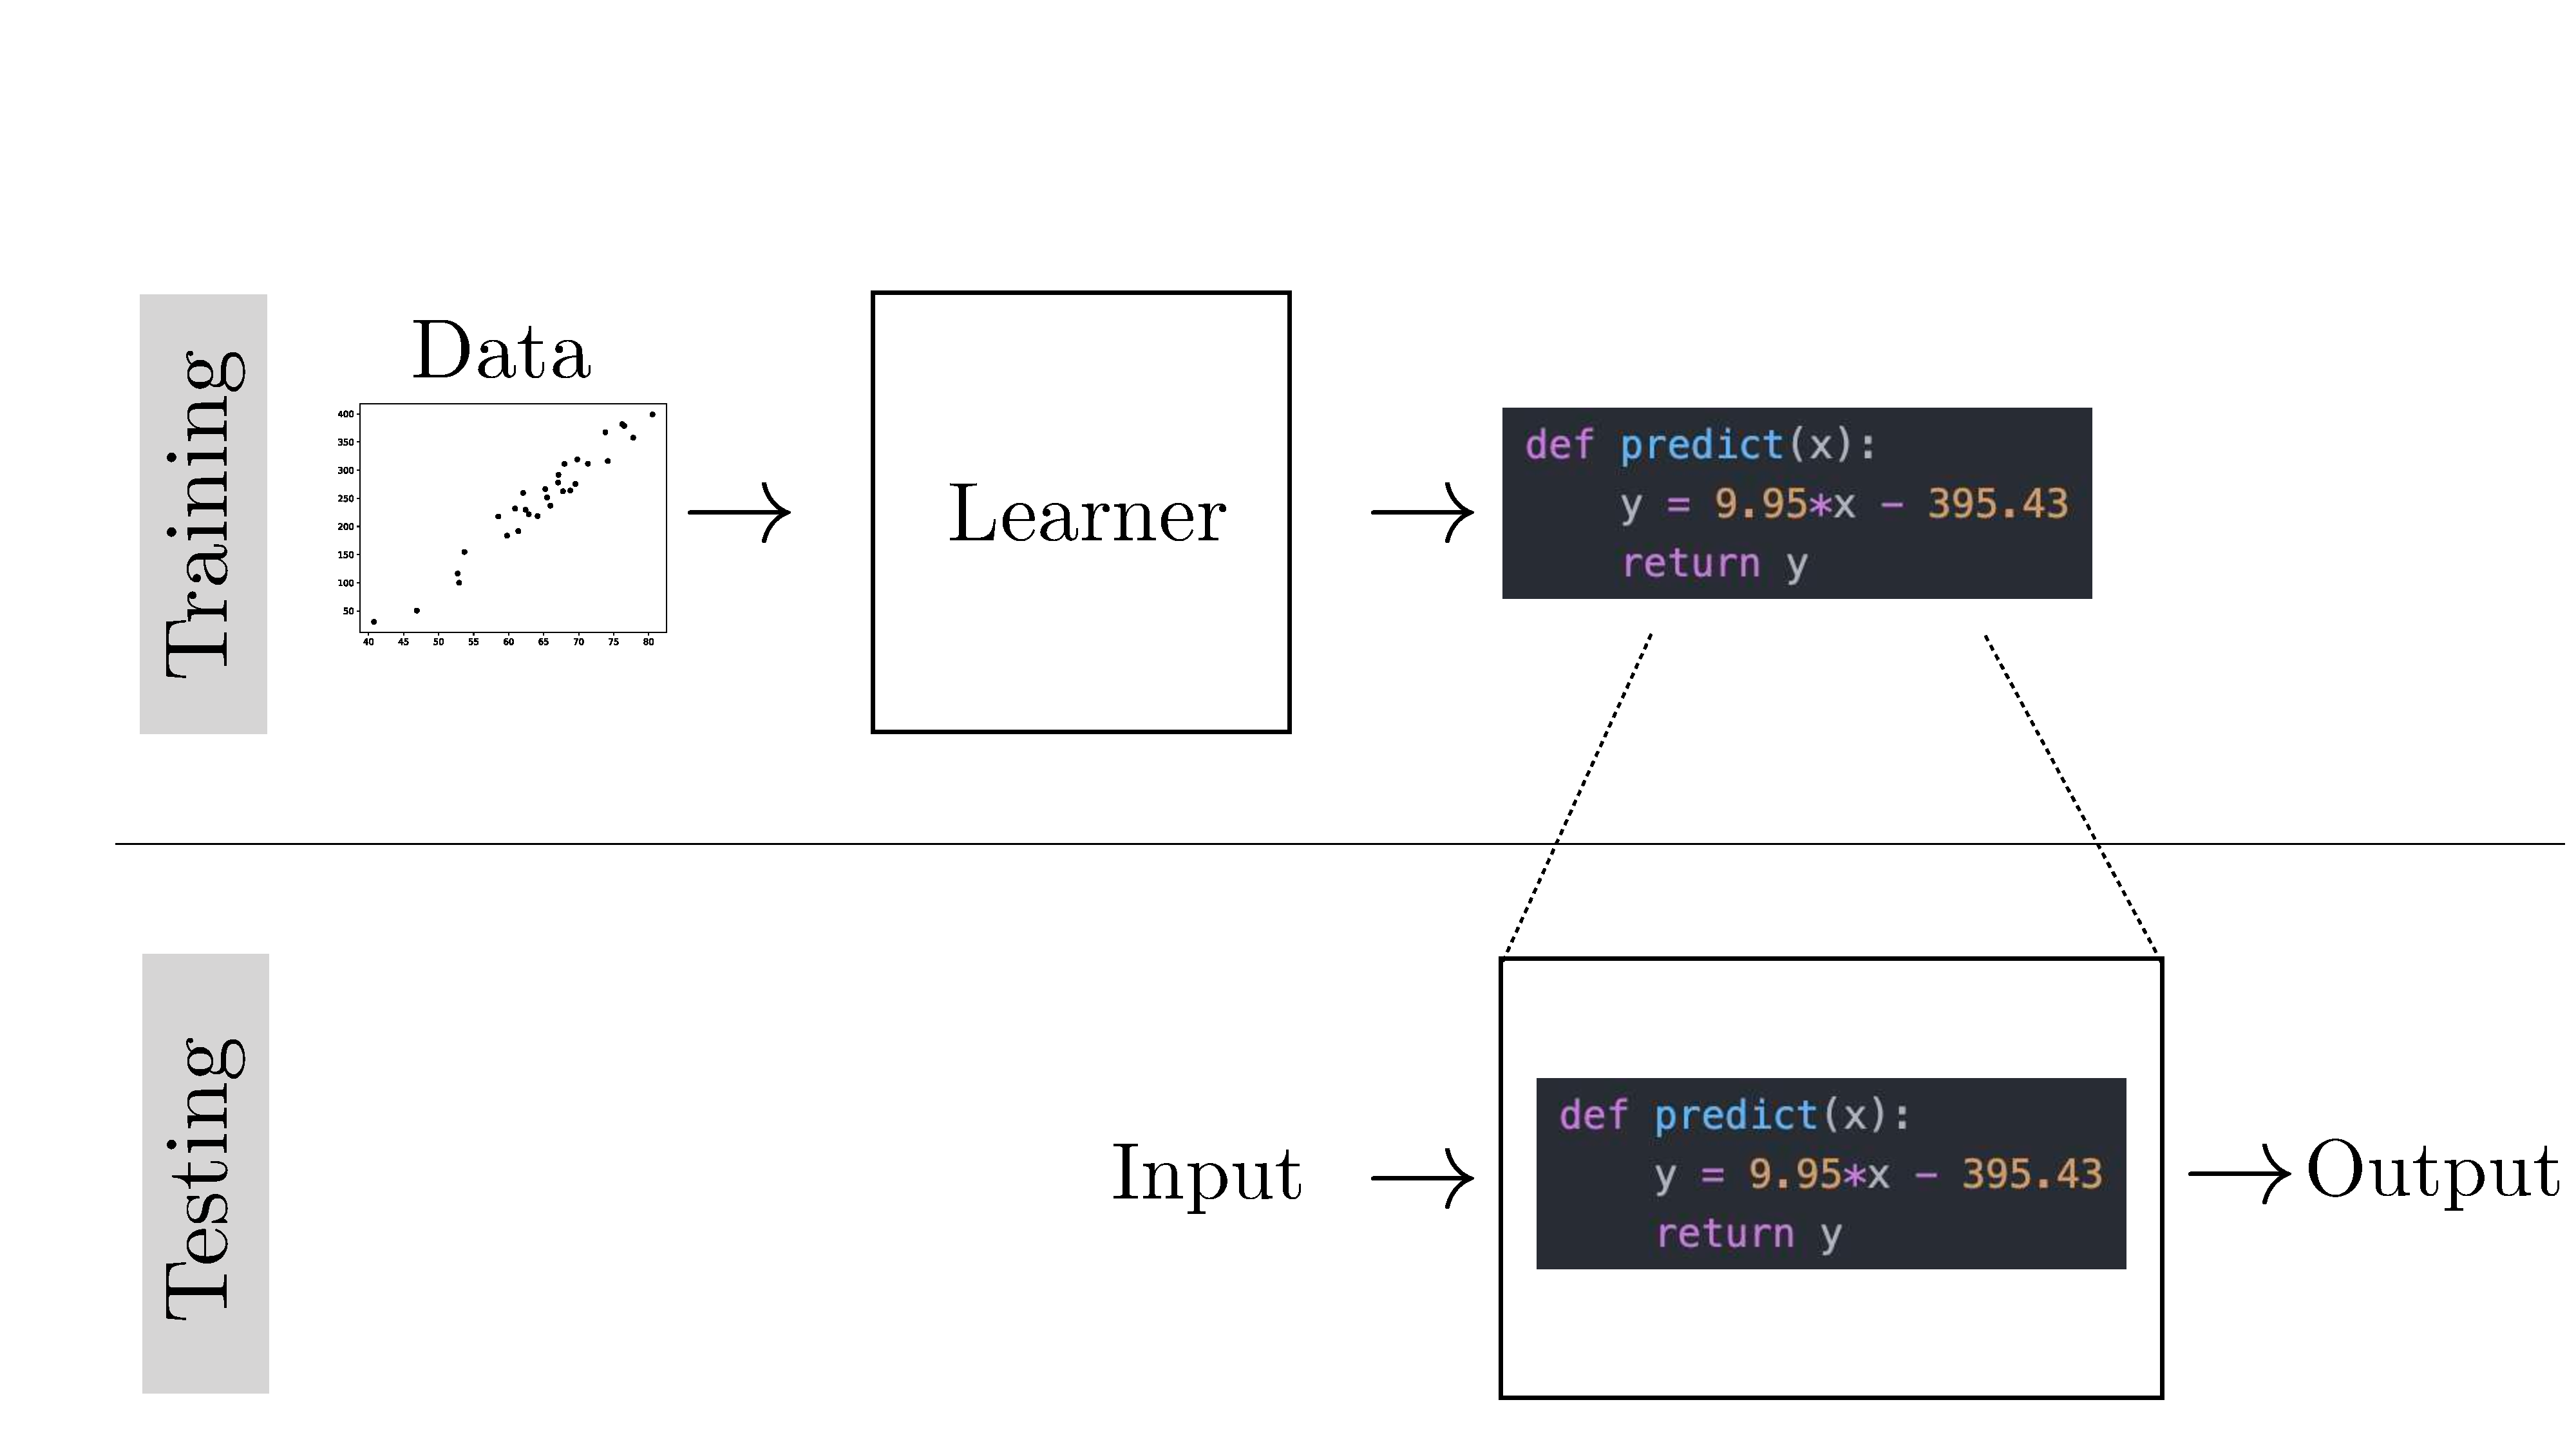
\includegraphics[width=0.8\linewidth]{./figures/intro_to_learning/program_induction_system_diagram.pdf}
    }
    \caption{Python program induction finds a Python program that predicts the training data's $y$-values from its $x$-values.}
    \label{fig:intro_to_learning:program_induction_system_diagram}
\end{figure}

\subsection{Example 3: Classification and Softmax Regression}\label{sec:intro_to_learning:image_classification}

A common problem in computer vision is to recognize objects. This is a \index{Classification}{\bf classification} problem. Our input is an image $\mathbf{x}$, and our target output is a class label $\mathbf{y}$ (\fig{\ref{fig:intro_to_learning:image_classification}}).

\begin{figure}[h]
    \centerline{
    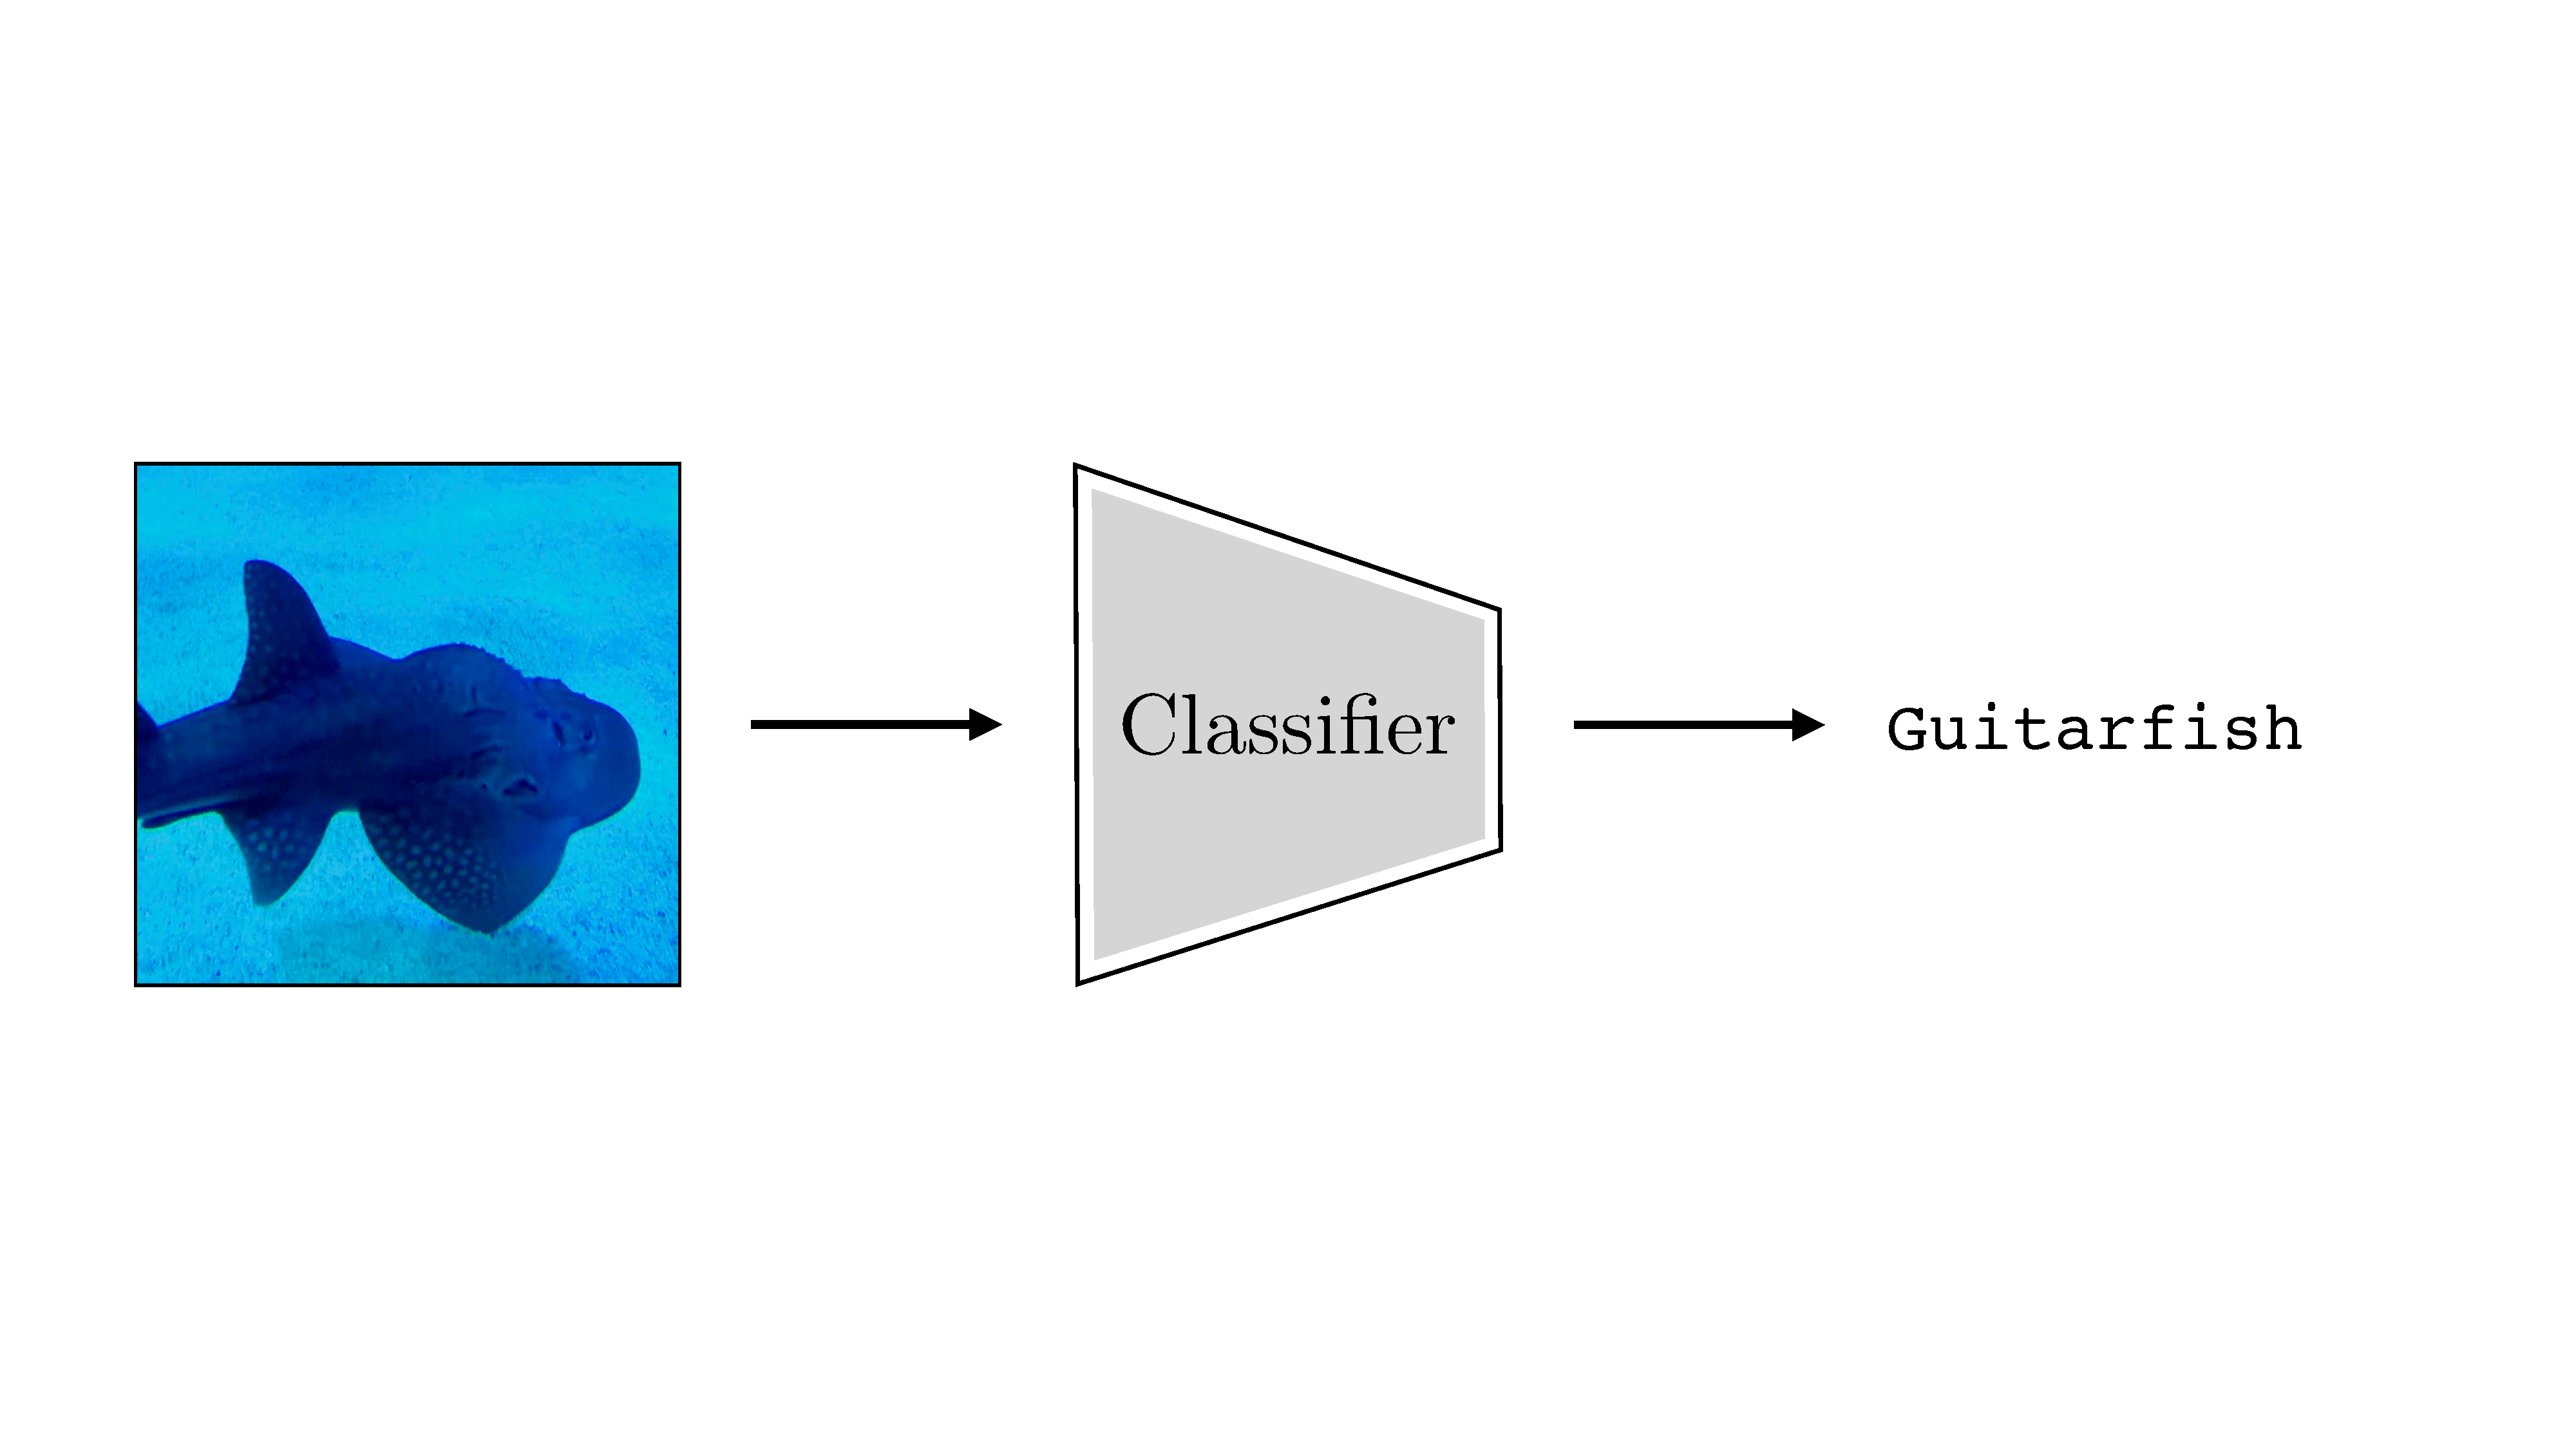
\includegraphics[width=0.7\linewidth]{./figures/intro_to_learning/image_classification.pdf}
    }
    \caption{Image classification.}
    \label{fig:intro_to_learning:image_classification}
\end{figure}

How should we formulate this task as a learning problem? The first question is how do we even represent the input and output? Representing images is pretty straightforward; as we have seen elsewhere in this book, they can be represented as arrays of numbers representing red-green-blue colors: $\mathbf{x} \in \mathbb{R}^{H \times W \times 3}$, where $H$ is image height and $W$ is image width.

How can we represent class labels? It turns out a convenient representation is to let $\mathbf{y}$ be a $K$-dimensional vector, for $K$ possible classes, with $y_k = 1$ if $\mathbf{y}$ represents class $k$, and $y_k = 0$ otherwise. This representation is called a \index{One-hot code}\textbf{one-hot code}, since just one element of the vector is on (``hot''). Each class has a unique one-hot code. We will see why this representation makes sense shortly. The one-hot codes are the targets for the function we are learning. Our goal is to learn a function $f_{\theta}$ that output vectors $\hat{\mathbf{y}}$ that match the one-hot codes, thereby correctly classifying the input images.
%So the learning problem is to map $f_{\theta}: \mathbb{R}^{H \times W \times 3} \rightarrow \mathbb{R}^K$. 
\marginnote{An example of one-hot codes for representing $K$=5 different classes:
\\[6pt]
\centerline{
\includegraphics[width=0.275\linewidth]{figures/intro_to_learning/one_hot_codes_white.eps}
}
}[-1.8cm]

Next, we need to pick a loss function. Our first idea might be that we should minimize misclassifications. That would correspond to the so called \index{0-1 loss}{\bf 0-1 loss}:
\begin{align}
    \mathcal{L}(\hat{\mathbf{y}},\mathbf{y}) = \mathbbm{1}(\hat{\mathbf{y}}\neq\mathbf{y}),
\end{align}
where $\mathbbm{1}$ is the indicator function that evaluates to 1 if and only if its argument is true, and 0 otherwise. Unfortunately, minimizing this loss is a discrete optimization problem, and it is NP-hard. Instead, people commonly use the \index{Cross-entropy loss}{\bf cross-entropy loss}, which is continuous and differentiable (making it easier to optimize):
\begin{align}
    \mathcal{L}(\hat{\mathbf{y}},\mathbf{y}) = H(\mathbf{y}, \hat{\mathbf{y}}) = - \sum_{k=1}^K y_k \log \hat{y}_k \quad\quad \triangleleft \quad \text{cross-entropy loss}
\end{align}
The way to think about this is $\hat{y}_k$ should \textit{represent the probability} we think the image is an image of class $k$. Under that interpretation, minimizing cross-entropy maximizes the log likelihood of the ground truth observation $\mathbf{y}$ under our model's prediction $\hat{\mathbf{y}}$.

For that interpretation to be valid, we require that $\hat{\mathbf{y}}$ represent a \index{Probability mass function}{\bf probability mass function} ({\bf pmf}). A pmf $\mathbf{p}$, over $K$ classes, is defined as a $K$-dimensional vector with elements in the range $[0,1]$ that sums to 1. In other words, $\mathbf{p}$ is a point on the $(K-1)$-\textbf{simplex}, which we denote as \index{Simplex}$\mathbf{p} \in \vartriangle^{K-1}$.\marginnote{The $(K-1)$-simplex, $\vartriangle^{K-1}$, is the set of all $K$-dimensional vectors whose elements sum to 1. $K$-dimensional one-hot codes live on the vertices of $\vartriangle^{K-1}$.}[-1.0cm]

To ensure that the output of our learned function $f_{\theta}$ has this property, i.e., $f_{\theta} \in \vartriangle^{K-1}$, we can compose two steps: (1) first apply a function $z_{\theta}: \mathcal{X} \rightarrow \mathbb{R}^K$, (2) then squash the output into the range $[0,1]$ and normalize it to sum to 1. 
%So, if our parameterized function outputs a vector $f_{\theta}(\mathbf{x}) \in \mathbb{R}^K$, then we can convert it to a pmf by squashing it into the range $[0,1]$ and normalizing it to sum to 1. 
A popular way to squash is via the \index{Softmax}{\bf softmax} function:\marginnote{Using softmax is a modeling choice; we could have used any function that squashes into a valid pmf, that is, a nonnegative vector that sums to 1.}[0.8cm]
\begin{align}
    &\mathbf{z} = z_{\theta}(\mathbf{x})\\
    &\hat{\mathbf{y}} = \texttt{softmax}(\mathbf{z})\\
    &\quad \quad \hat{y}_j = \frac{e^{-z_j}}{\sum_{i=1}^K e^{-z_k}}.
\end{align}
The values in $\mathbf{z}$ are called the \index{Logits}\textbf{logits} and can be interpreted as the unnormalized log probabilities of each class. 
Now we have,
\begin{align}
    \hat{\mathbf{y}} = f_{\theta}(\mathbf{x}) = \texttt{softmax}(z_{\theta}(\mathbf{x}))
\end{align}
\Fig{\ref{fig:softmax_regression_diagram}} shows what the variables look like for processing one photo of a fish during training.

\begin{figure}[h]
    \centering
    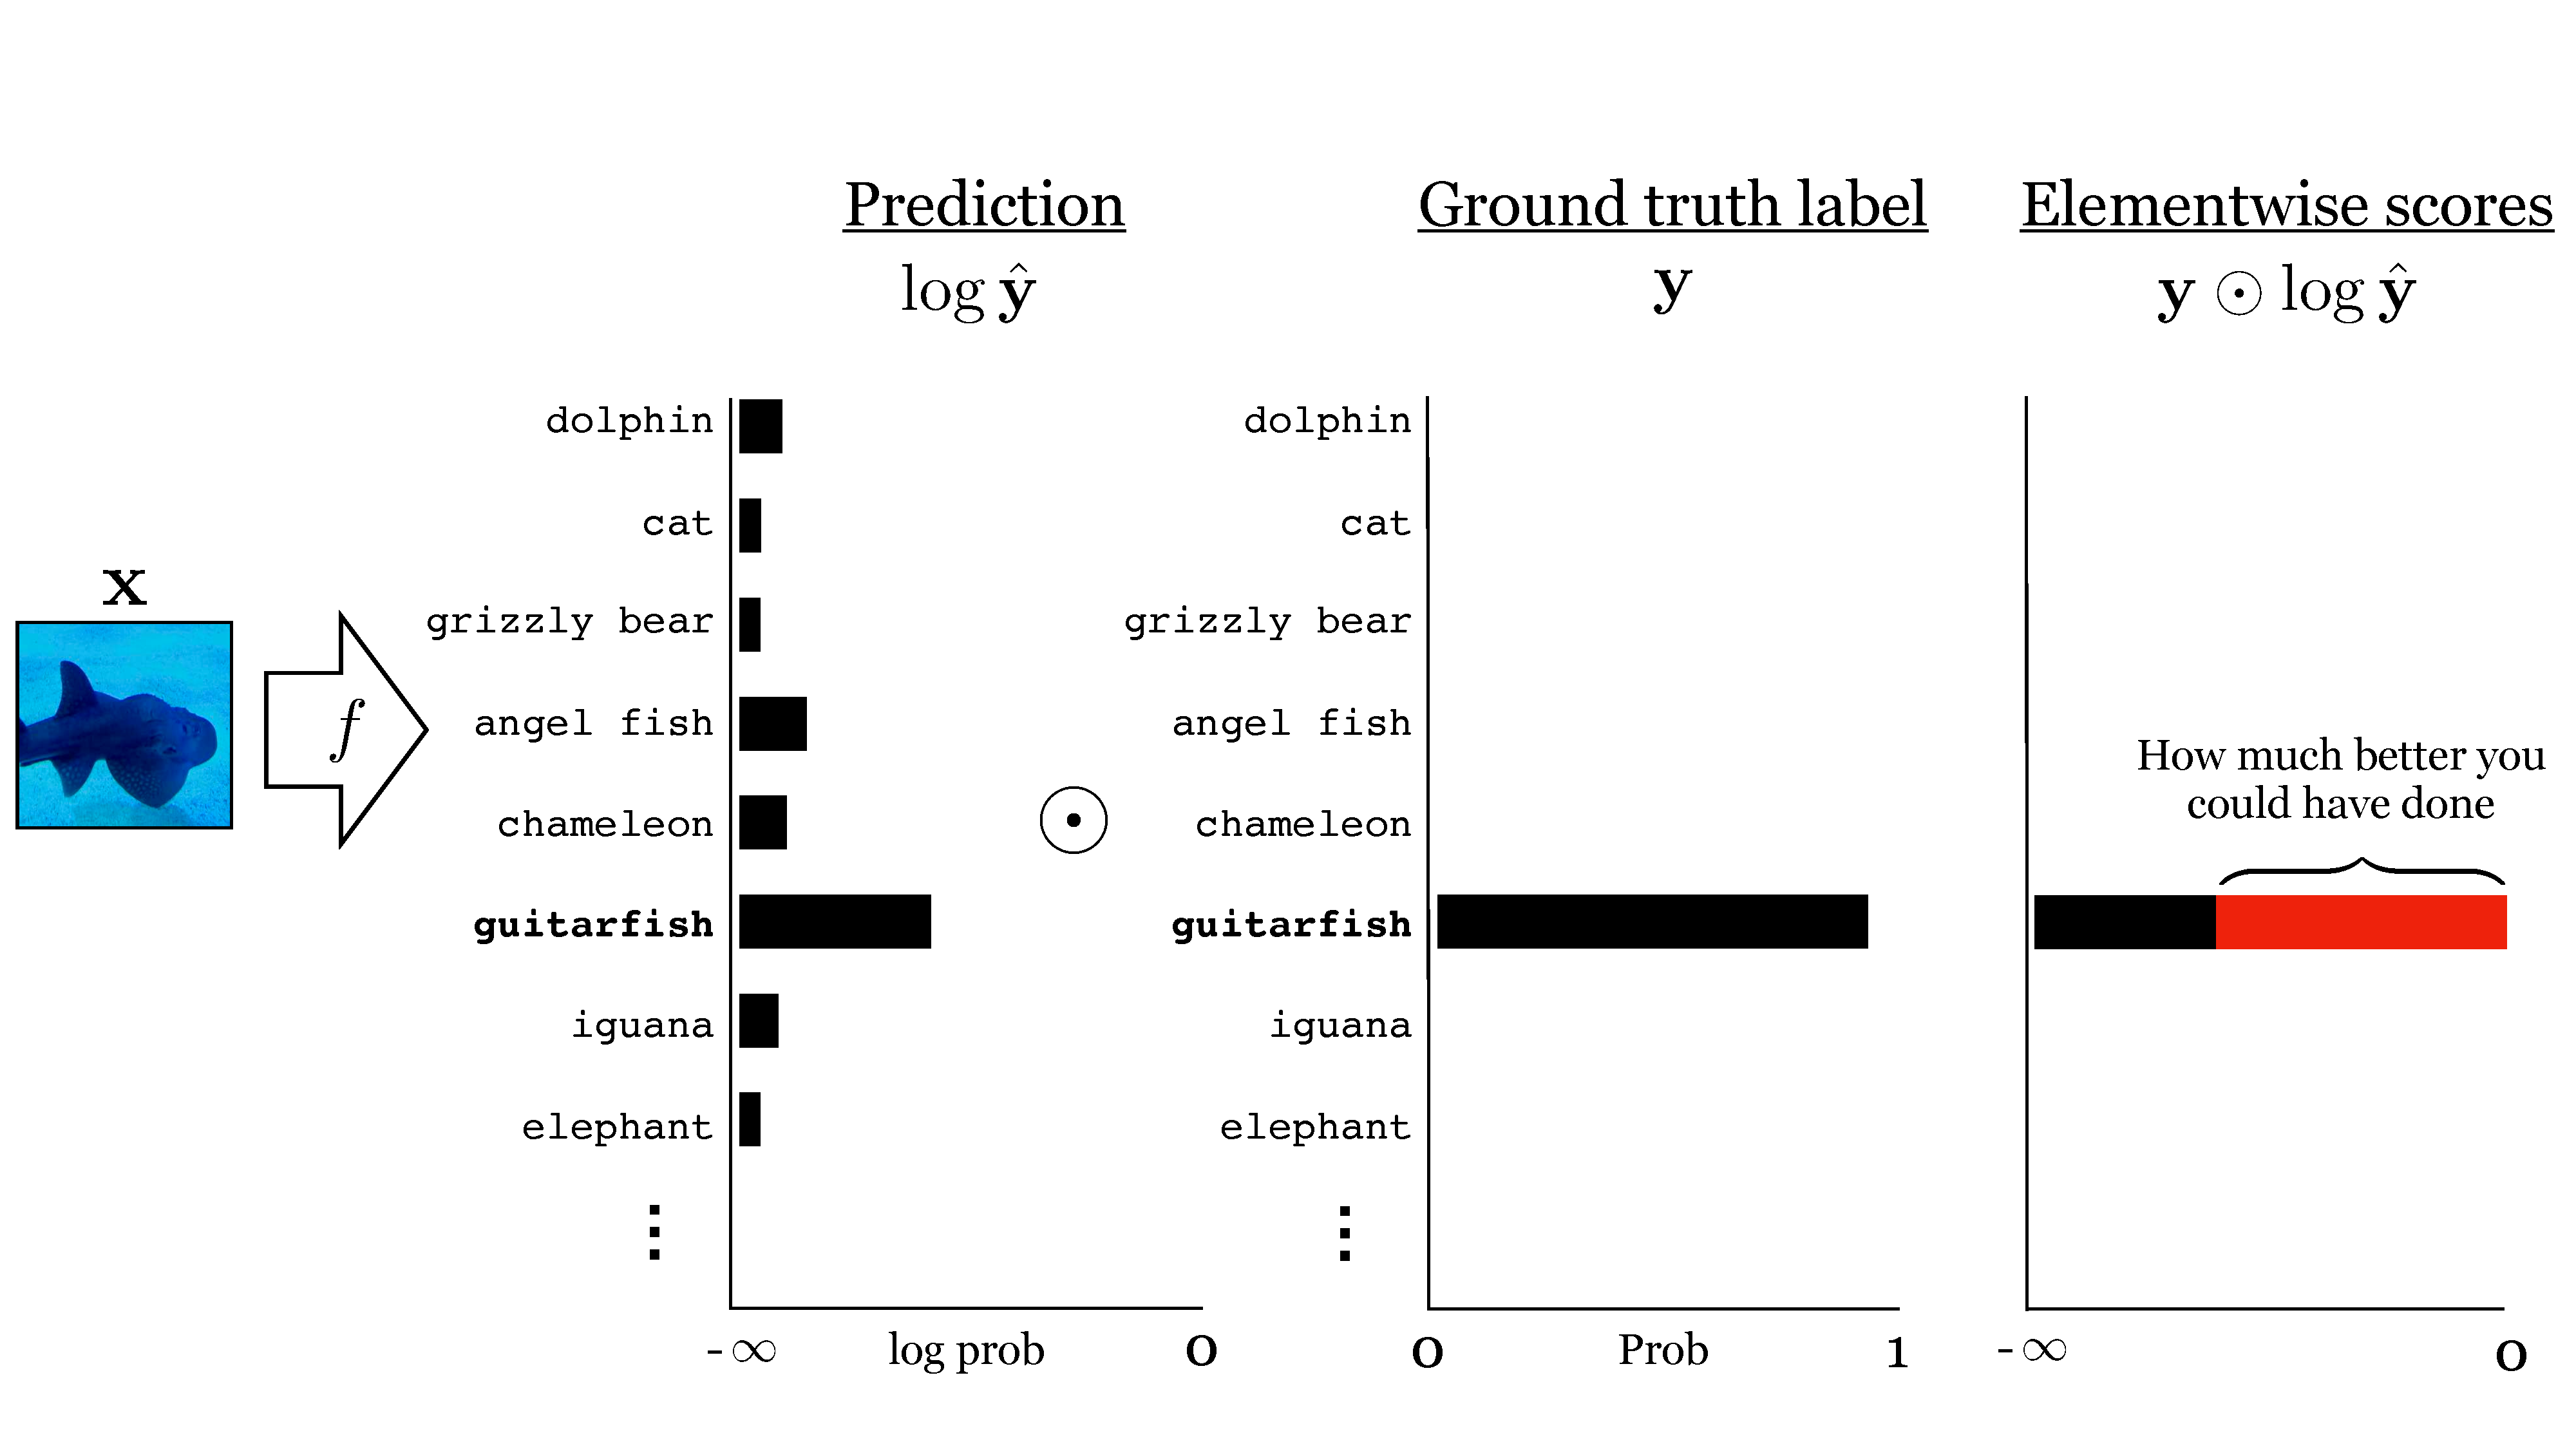
\includegraphics[width=1.0\linewidth]{./figures/intro_to_learning/softmax_regression_diagram.pdf}
    \caption{Softmax regression for image classification. The $\odot$ symbol represents an elementwise product. The cross-entropy loss is the negative of the sum over elementwise agreements between the prediction vector $\hat{\mathbf{y}}$ and the label vector $\mathbf{y}$, that is, if $\mathbf{s} = \mathbf{y} \odot \log \hat{\mathbf{y}}$ is the vector of scores for how well our prediction agrees with the label, then our cross-entropy loss is $H(\mathbf{y}, \hat{\mathbf{y}}) = - \sum_{k=1}^K s_k$.}
    \label{fig:softmax_regression_diagram}
\end{figure}

The prediction placed about 40 percent probability on the true class, ``guitarfish,'' so we are 60 percent off from an ideal prediction (indicated by the red bar; an ideal prediction would place 100 percent probability on the true class). Our loss is $-\log 0.4$.

This learning problem, which is also called \index{Softmax regression}{\bf softmax regression}, can be summarized as follows:\marginnote{Softmax regression is just one way to model a classification problem. We could have made other choices for how to map input data to class labels.}[-0.4cm]

\begin{center}
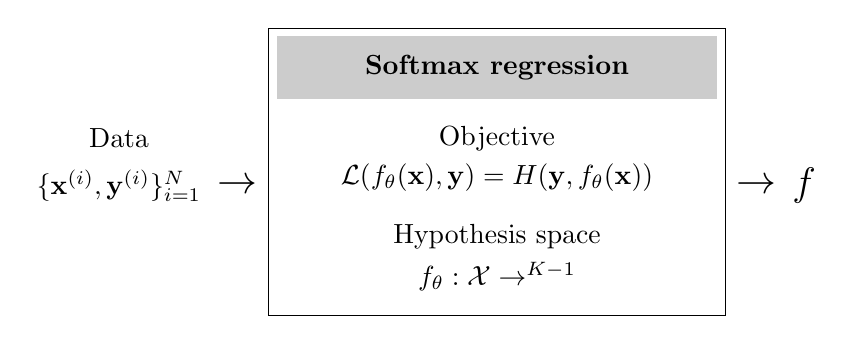
\begin{tikzpicture}
    \draw (0,-1.25) rectangle (5.8,2.4); % outer box
    \fill[black!20] (0.1,1.5) rectangle (5.7,2.3); % gray box
    \node[] at (2.9,1.9) {{\bf Softmax regression}};
    \node[] at (2.9,1.0) {Objective}; \node[] at (2.9,0.5) {$\mathcal{L}(f_{\theta}(\mathbf{x}), \mathbf{y}) = H(\mathbf{y}, f_{\theta}(\mathbf{x}))$};
    \node[] at (2.9,-0.25) {Hypothesis space}; \node[] at (2.9,-0.75) {$f_{\theta}: \mathcal{X} \rightarrow \vartriangle^{K-1}$};
    \node[] at (-1.9,1.0) {Data};
    \node[] at (-1.9,0.4) {$\{\mathbf{x}^{(i)}, \mathbf{y}^{(i)}\}_{i=1}^N$};
    \node[] at (-0.4,0.4) {{\Large  $ \rightarrow$}};
    \node[] at (6.8,0.4) {{\Large $f$}};
    \node[] at (6.2,0.4) {{\Large  $ \rightarrow$}};
\label{fig:softmax_regression_learning_problem}
\end{tikzpicture}
\end{center}
% \begin{figure}[h]
%     \centering
%     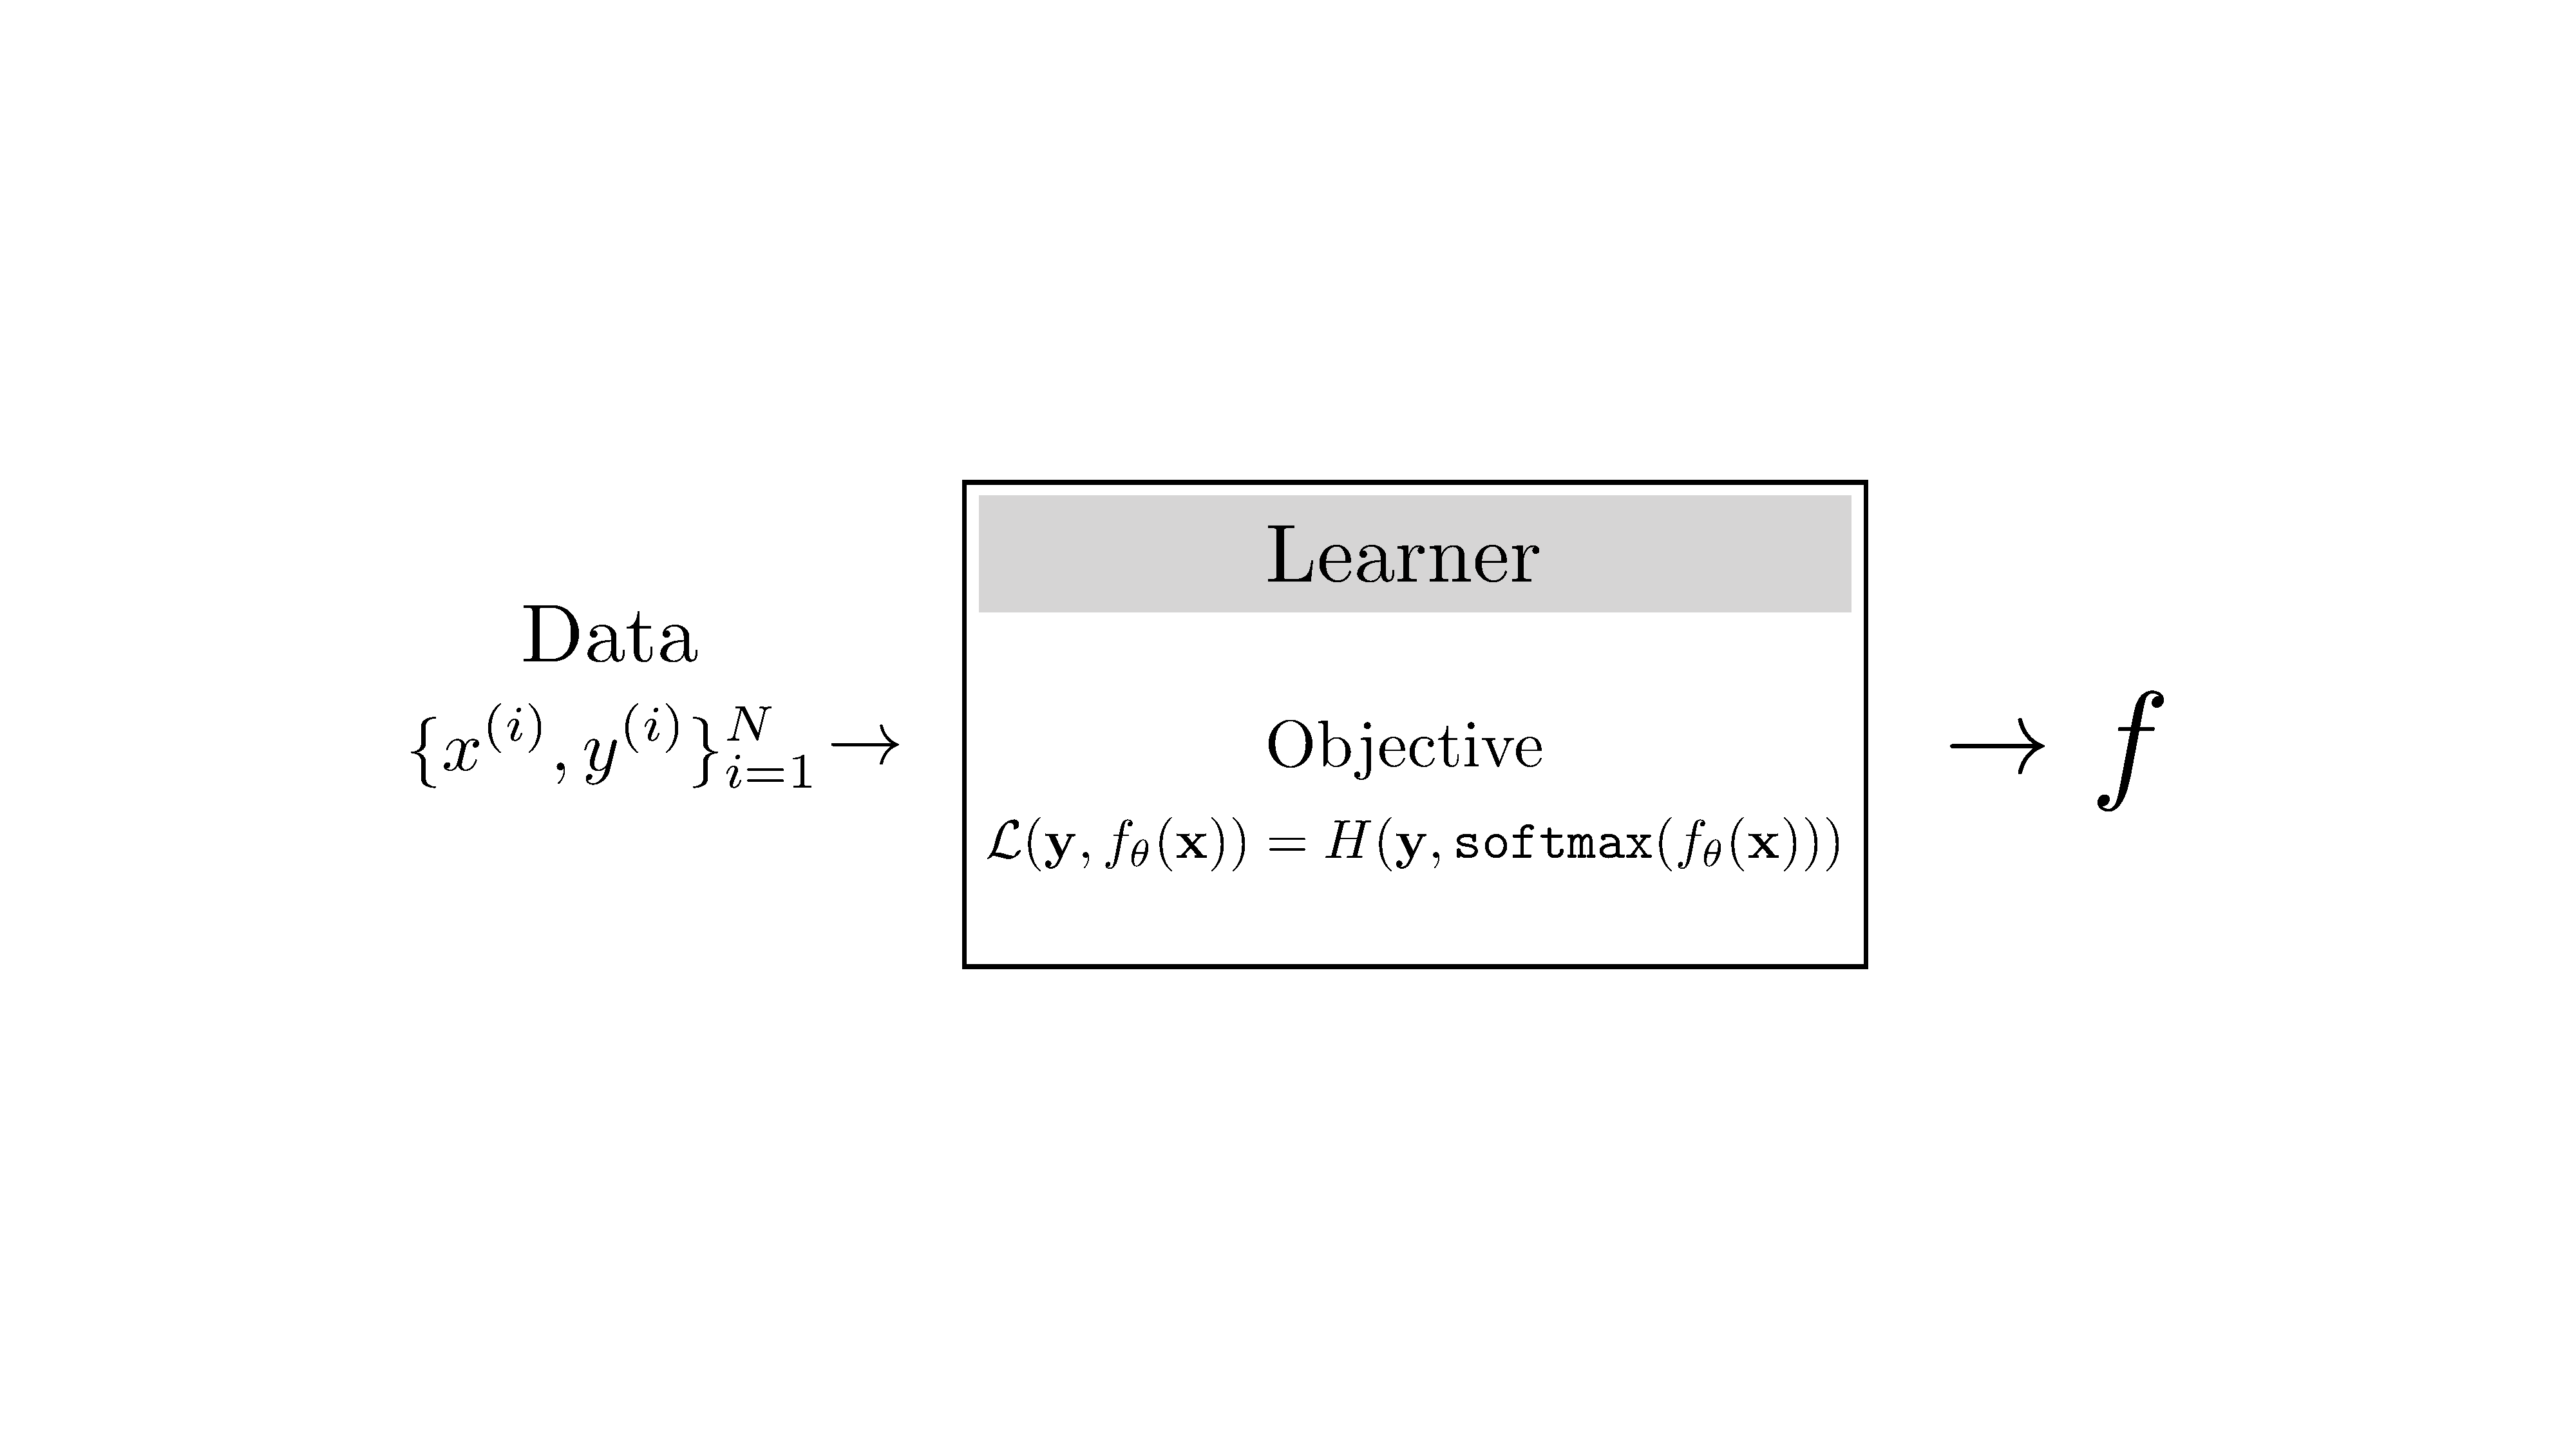
\includegraphics[width=0.7\linewidth]{./figures/intro_to_learning/softmax_regression_learning_problem.pdf}
%     \label{fig:softmax_regression_learning_problem}
% \end{figure}
Notice that we have left the hypothesis space only partially specified, and we left the optimizer unspecified. This is because softmax regression refers to the whole family of learning methods that have this general form. This is one of the reasons we conceptualized the learning problem in terms of the three key ingredients described previously: you can often develop them each in isolation, then mix and match.

%\#1 specifies the ``hypothesis space" (aka ``model class") we will search over. A simple model class would be ``linear functions". A more complex model class might be ``C++ programs". \#2 specifies the ``objective function" we wish to optimize. Suppose we are trying to predict tomorrow's weather. Then a natural objective would be that our prediction is close to the truth, for example, we could measure the Euclidean distance between our prediction of the temperature and what its actual value turns out to be. If we use linear functions for our model class, and Euclidean distance for our objective function, then we get what is known as a ``linear least squares" problem. 

%The final question, \#3, is how do we search over the model class to find the instantiation that optimizes the objective? One common approach is hill climbing: starting with some initial parameters, adjust them slightly in the direction that locally improves the objective. Hill climbing can be done by trial and error -- make random adjustments and keep the ones that improved the score -- or by gradient ascent -- use the derivative of the objective function with respect to the parameters to determine the adjustment that will locally increase the objective the most.

%For most of the rest of this class, we will consider machine learning algorithms that answer these three questions as follows:
%\begin{enumerate}
%    \item Hypothesis space: deep neural nets
%    \item Objective: predictions should be close to the truth
%    \item Optimizer: gradient descent
%\end{enumerate}

%What remains is to investigate each of these components in detail.



%\section{Reinforcement learning}
%{\bf Reinforcement learning} is a term that means many different things to different people. A classic definition is learners whose objective is to optimize a {\bf reward function}, rather than to fit a model to examples. A reward function is a mapping from outputs to scores: $r: Y \rightarrow \mathbb{R}$. The learning tries to come up with a function that maximizes rewards.

%However, there is another special distinction of reinforcement learning, and in my opinion a more important distinction: reinforcement learning deals with the setting where data is a function of the learned policy.

%\marginnote{In fact, most terms in machine learning do not have precise, agreed upon definitions. Instead they refer to a collection of connotations, and these connotations will be different in different communities.}[-1.83cm]

%\section{Unsupervised learning}


\section{Learning to Learn}% {\small [Advanced topic]}}

Learning to learn, also called \index{Metalearning}{\bf metalearning}, is a special case of learning where the hypothesis space is learning algorithms. 

Recall that learners train on past instances of a problem to produce an algorithm that can solve future instances of the problem. The goal of metalearning is to handle the case where the future problem we will encounter is itself a learning problem, such as ``find the least-squares line fit to these data points.'' One way to train for this would be by example. Suppose that we are given the following \{\texttt{input}, \texttt{output}\} examples:
\begin{align}
    &\{\texttt{input:} \big(x:[1,2], y:[1,2]\big), &&\texttt{output:} y = x\}\nonumber \\
    &\{\texttt{input:} \big(x:[1,2], y:[2,4]\big), &&\texttt{output:} y = 2x\}\nonumber \\
    &\{\texttt{input:} \big(x:[1,2], y:[0.5,1]\big), &&\texttt{output:} y = \frac{x}{2}\}\nonumber
\end{align}
These are examples of performing least-squares regression; therefore the learner can fit these examples by learning to perform least-squares regression.\marginnote{Note that least-squares regression is not the unique solution that fits these examples, and the metalearner might arrive at a different solution that fits equally well.}[-0.8cm] Since least-squares regression is itself a learning algorithm, we can say that the learner learned to learn.

We started this chapter by saying the learning is a meta-algorithm: it's an algorithm that outputs an algorithm. Metalearning is a meta-meta-algorithm and we can visualize it by just adding another outer loop on top of a learner, as shown in \fig{\ref{fig:intro_to_learning:meta_learning_diagram}}.
\begin{figure}[h]
    \centerline{
    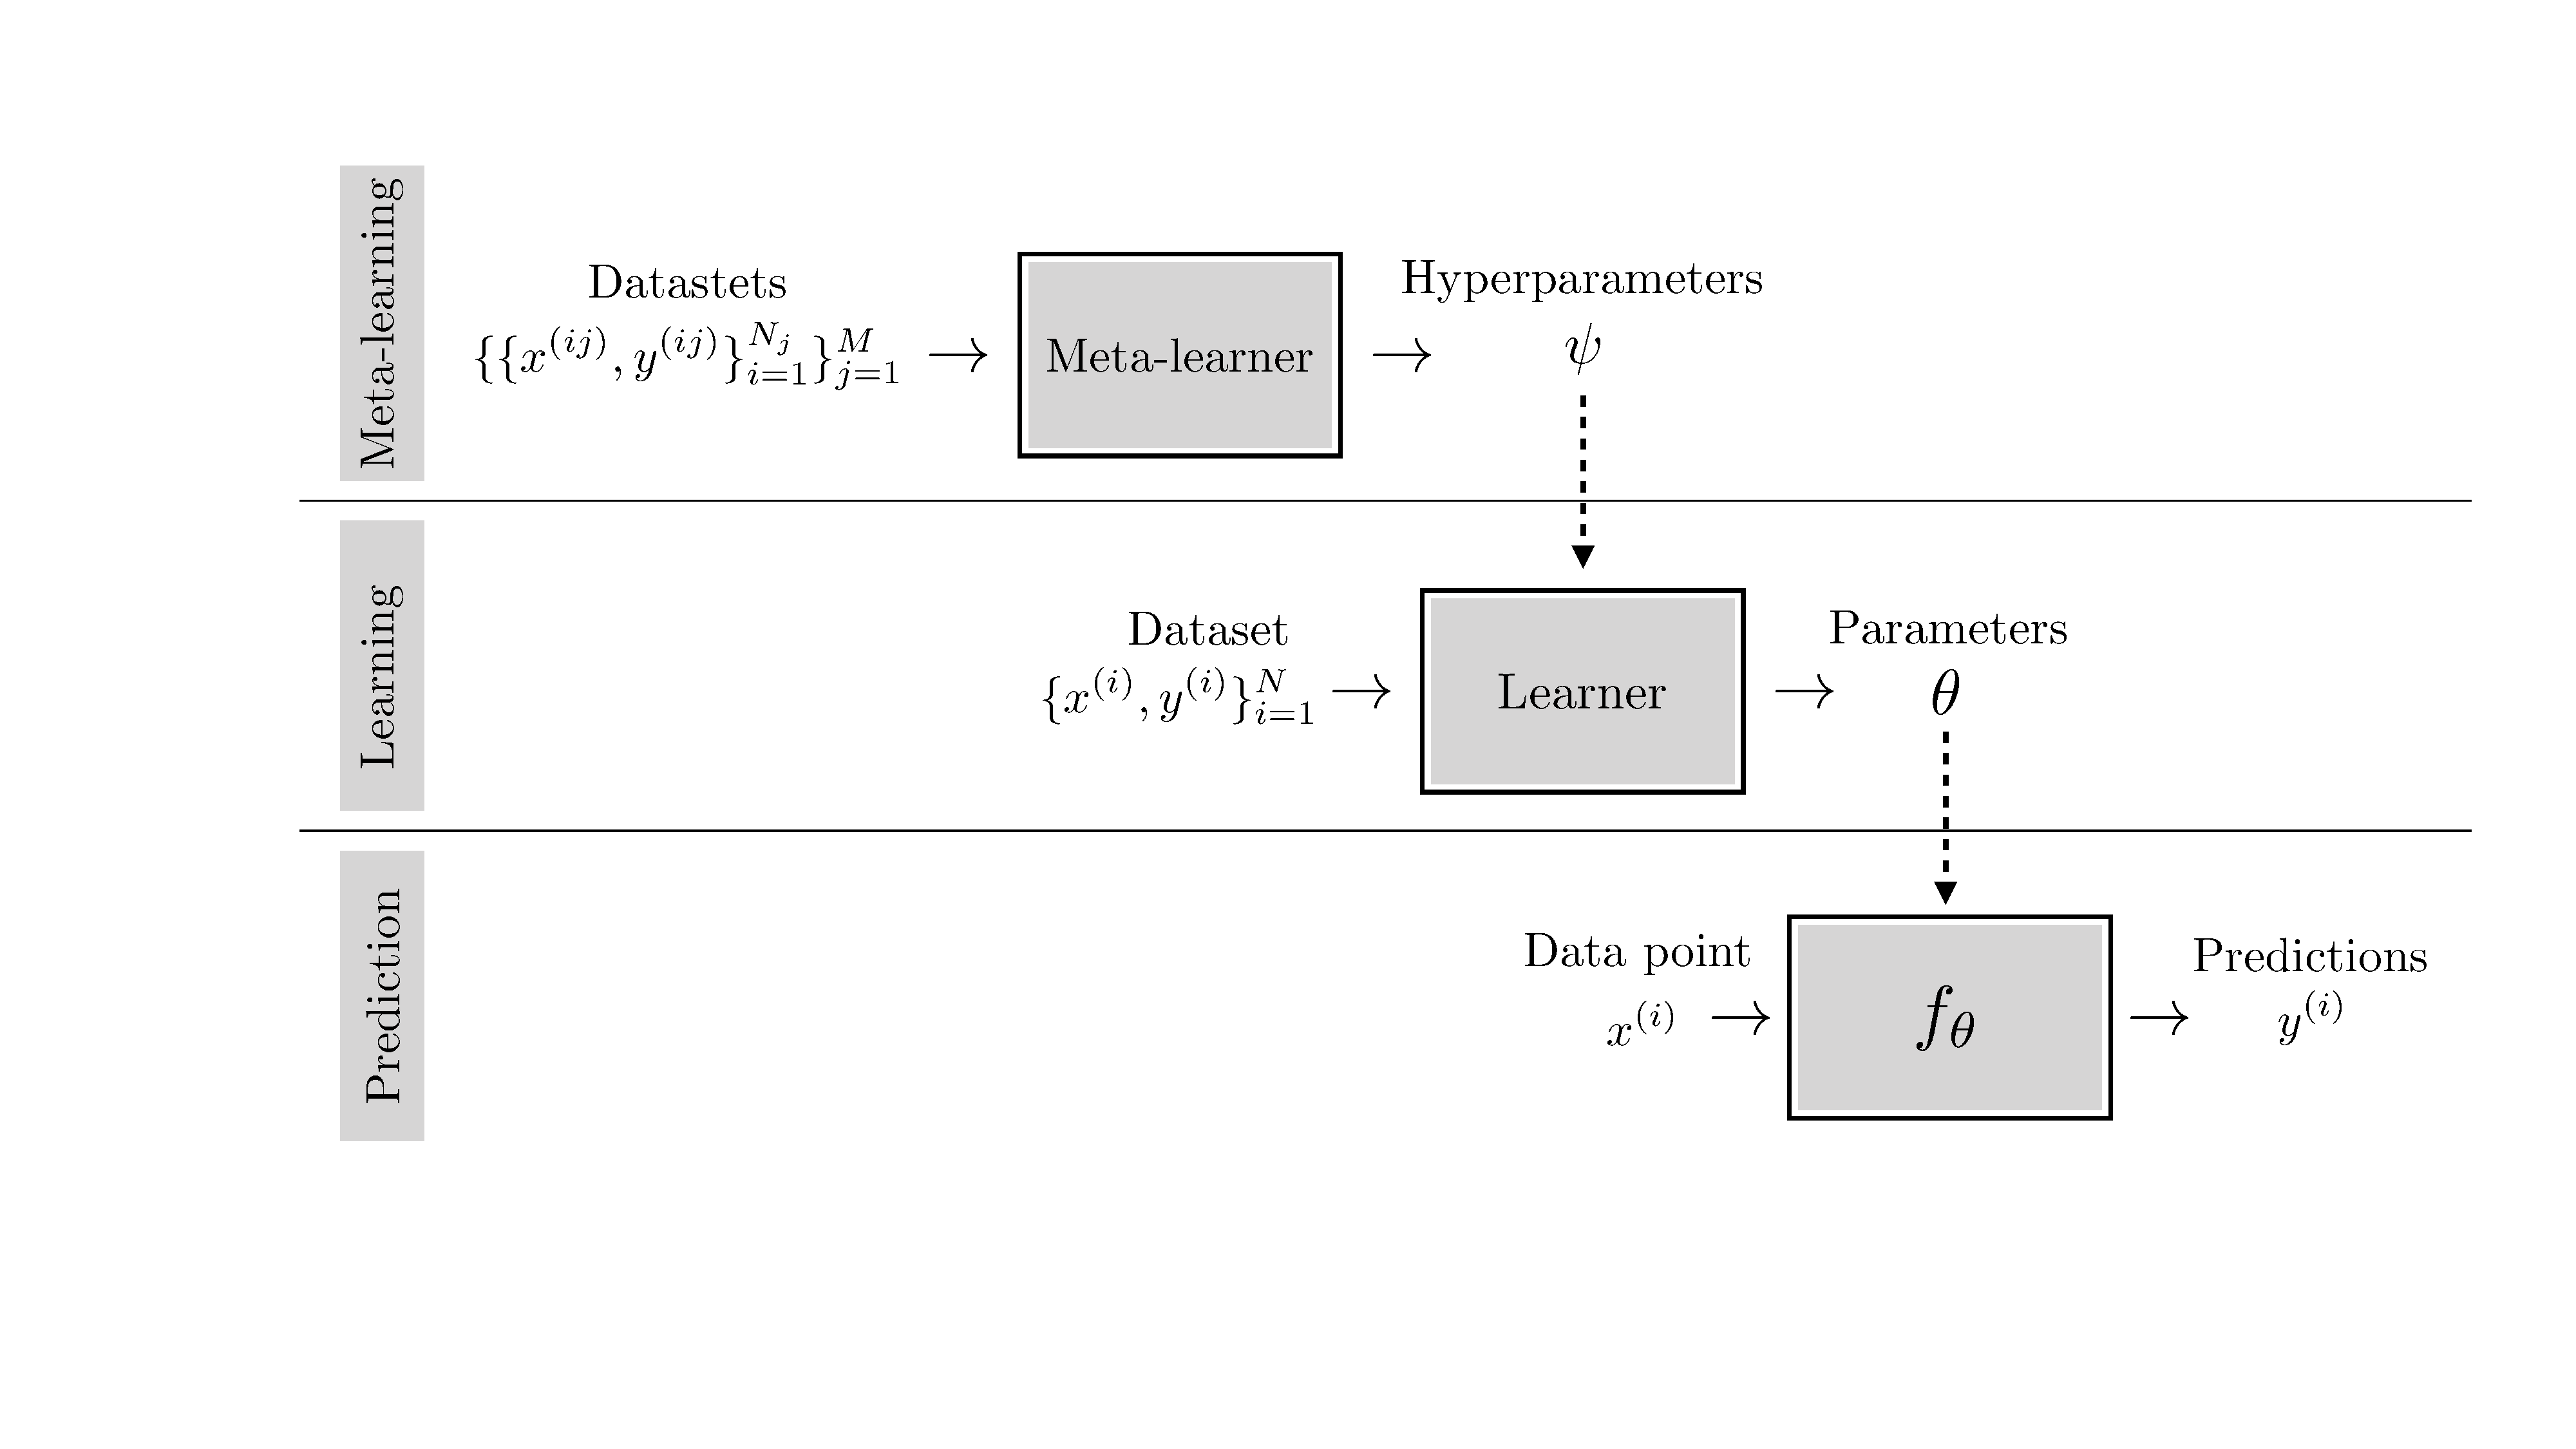
\includegraphics[width=1.0\linewidth]{./figures/intro_to_learning/meta_learning_diagram.pdf}
    }
    \caption{Learning is a meta-algorithm, an algorithm that outputs algorithms; metalearning is just learning applied to learning, and therefore it is a meta-meta-algorithm.}
    \label{fig:intro_to_learning:meta_learning_diagram}
\end{figure}

Notice that you can apply this idea recursively, constructing meta-meta-...-metalearners. Humans perform at least three levels of this process, if not more: we have \emph{evolved} to be \emph{taught} in school how to \emph{learn} quickly on our own.
\marginnote{{\bf Evolution} is a learning algorithm according to our present definition.}[-1.0cm]

\section{Concluding Remarks}
Learning is an extremely general and powerful approach to problem solving. It turns data into algorithms. In this era of big data, learning is very often the preferred approach. It is a a major component of almost all modern computer vision systems.
